\chapter{\label{ch:3-orion}Attosecond X-ray harmonics on the ORION laser facility} 

\minitoc

\section{Introduction}
The simulations of Chapter \ref{ch:2-zvp} are a relatively efficient and cost-effective mode of study. In comparison, high-power laser experiments are a cumbersome and technical challenge. However, the proliferation of errors in simulation codes leads to their inevitable deviation from reality, while reality itself diverges from the idealised conditions of the codes. For now, at least, experiments remain an essential component of the scientific method. This chapter reports on the March 2023 experiment at the ORION laser facility, AWE, Aldermaston, the UK's most powerful laser system. The pulse duration is too long to create the attosecond electron bunches of the previous chapter. Instead, this chapter focuses on the ROM model of HHG. This model describes the properties of radiation reflected from a relativistic laser pulse interaction with a solid-density plasma, another related route to bright attosecond light sources. 

A fundamentally different mechanism to its Nobel prize-winning counterpart, SHHG from solids has demonstrated significantly higher conversion efficiencies and, relying on plasma oscillations not ionisation, does not suffer from the same limits to applied intensity \cite{teubnerHighorderHarmonicsLaserirradiated2009}. SHHG has thus become a field of considerable interest for the production of bright coherent attosecond harmonics. First observed from the interaction of a CO$_2$ laser-solid interaction in 1981 \cite{carmanVisibleHarmonicEmission1981} and followed shortly by a theoretical justification \cite{bezzeridesPlasmaMechanismUltraviolet1982}, interest in HHG was revived by the arrival of CPA technology enabling access to unprecedented laser pulse intensities. To describe this new relativistic interaction, 1994 saw the arrival of a new theory, the \ac{OMM} \cite{bulanovInteractionUltrashortRelativistically1994}. Harmonic of the incident laser pulse were seen to be formed by the Doppler effect induced by a thin reflecting charge sheet at the plasma surface oscillating periodically with the laser pulse. This theory predicts a cutoff harmonic number of $n_\mathrm{c} = 4\gamma_\mathrm{s}^2 $, where $\gamma_\mathrm{s}$ is the maximum gamma factor of the charge sheet. This relatively low cutoff is at odds with experimental results, the current record standing at the 3200\th harmonic observed on the Vulcan PW laser system in 2007 \cite{dromeyBrightMultikeVHarmonic2007}. It was only after the development of relativistic similarity theory \cite{gordienkoScalingsUltrarelativisticLaser2005}, which laid the groundwork for Baeva's ROM model, that the experimentally observed cut-off could now be explained \cite{baevaTheoryHighorderHarmonic2006}. Since ORION and Vulcan parameter spaces are similar, this is the most appropriate description of SHHG and is described in more detail in Section \ref{ch:3-sec:theory}.

There are many fascinating applications for SHHG beyond that of attosecond physics. The high photon energy content of the harmonic beam has excellent penetration into dense materials with preliminary studies indicating notable improvement in energy absorption, suitable for auxiliary heating of ICF targets \cite{paddockEnergyGainWettedfoam2024}. This high energy content also enables the focusing of the harmonic beam to significantly smaller spot sizes than the incident diffraction-limited laser pulse. An all-optical coherent focusing of high harmonics with realistic laser parameters has been shown to produce over 1000 times intensity gain \cite{vincentiAchievingExtremeLight2019}, thus providing a realistic route to the Schwinger limit \cite{quereReflectingPetawattLasers2021}. Such a beam could have potential for enhancing the signal of photon-photon scattering \cite{aboushelbayaOrbitalAngularMomentum2019} or of gravitational waves from twisted light \cite{atongaGravitationalWavesHighpower2023}. Simulations have shown how a harmonic beam can probe \ac{SF-QED} if a solid target is placed at the new focal position \cite{fedeliProbingStrongfieldQED2020}.

This chapter reports on the March 2023 experimental campaign at ORION to observe and measure the absolute intensity of X-ray harmonics generated via ROM HHG. Section \ref{ch:3-sec:theory} covers the theory of the ROM model of HHG from relativistic laser solid interactions. Section \ref{ch:3-sec:simulations} presents simulation results that guided both experimental design and data analysis. The experimental design is covered in Section \ref{ch:3-sec:experiment}, in Section \ref{ch:3-sec:data_processing} the data analysis. Results are presented in Section \ref{ch:3-sec:results} that are then summarised in Section \ref{ch:3-sec:conclusion}. 

\section{\label{ch:3-sec:theory}Theory}
\subsection{The ROM model}
For the moderately relativistic sub-picosecond ORION SP1 and SP2 beamlines, the most appropriate description for their non-linear interaction with a solid density target is the Relativistic Oscillating Mirror (ROM) model. The full technical formulation constitutes the main body of Baeva's 2008 thesis \cite{baevaHighHarmonicGeneration2008}, a notably more rigorous derivation than the original paper on the same topic \cite{baevaTheoryHighorderHarmonic2006}. This is achieved via application of the highly generalised \ac{ARP} formalism to the case of $S>1$ in relativistic similarity theory, showing that the \ac{ARP} coincides with the relativistic critical density surface. This section provides a more qualitative, physically motivated description of this theory, the salient point of Baeva's thesis being that, while the surface motion is generally complex and parameter space dependent, at the short moment in time when most high harmonics are generated, the surface motion is always parabolic. By application of the Bourdier method, detailed in Appendix \ref{sec:app-bourdier} \cite{bourdierObliqueIncidenceStrong1983}, Baeva demonstrated that the envelope of the spectral content of the reflected beam does not deviate from the normal incidence linearly polarised case for either s- or p-polarised incidence. Hence, the following discussion is restricted to normal incidence. It begins with relativistic similarity theory and Equation \ref{{eq:intro-p_similarity}}, $\mathbf{p} \sim a_0$. As discussed in Section \ref{sec:zvp-intro}, microscopically electrons follow similar relativistic trajectories. However, from Equation \ref{eq:zvp-vprop}, $v_\mathrm{prop}$, the velocity of electrons along the propagation axis of the laser pulse, is not necessarily relativistic except at the passing of the zero of the vector potential where $v_\mathrm{prop} \to c$. Macroscopically, the well-defined critical density surface within the skin depth (located at $S =1$), has a gamma factor that tracks the electrons' velocity along the propagation direction ($x$-direction) at that point,
\begin{equation}\label{eq:orion-gamma_s}
	\gamma_\mathrm{s} = \frac{1}{\sqrt{1-v_\mathrm{prop}^2/c^2}} = \sqrt{ \frac{1 + a(t,x)^2 +  p_\mathrm{prop}^2/(m_\mathrm{e}c)^2}{1 + a(t,x)^2}}.
\end{equation}
Equation \ref{eq:orion-gamma_s} indicates surface gamma factors of order unity except at zeros in the vector potential where $\gamma_\mathrm{s} \sim a_0$. In the viscinity of the zero, $a \sim a_0\sin(\omega_L t) \approx a_0\omega_\mathrm{L}t$. Thus, while the velocity of the surface is a smoothly varying function around the maximum, $v_\mathrm{s,\, max} \sim 1 - \mathcal{O}(a_0^{-2})$, the \textit{gamma factor spikes} as the vector potential passes through zero. At this point, the surface emits high-frequency photons. The surface radiates such photons only in the vicinity of the gamma spike. Thus, the pulse width can be approximated. In ZVP theory, zeros overtake the emitted photons. Radiation from the extended electron bunch that is emitted first arrives at the observer last. In the ROM regime, Baeva demonstrates zeroes move at speed $c$. Consequently, all points in the skin depth radiate coherently. Since the radiation overtakes the sub-light speed surface, photons emitted from the surface first are observed first. The radiation emitted therefore has a duration of
\begin{equation}
	\Delta l \approx (c-|\mathbf{v}_\mathrm{s,\, max}|)\Delta t \approx \frac{\Delta t}{\gamma_\mathrm{s,\, max}^2},
\end{equation}
where $\Delta t$ is the temporal duration of the gamma spike. 

Writing the surface velocity as a smoothly varying function around its maximum,
\begin{equation}\label{eq:orion-vs}
	\mathbf{v}_\mathrm{s}(t) = -(v_\mathrm{s,\, max} - c\alpha(\omega_\mathrm{L}t)^2) \mathbf{\hat{x}}.
\end{equation}
Without loss of generality, the peak of the gamma spike is set to $t=0$ for cleaner notation. Around the gamma spike, the surface gamma factor is thus
\begin{equation}
	\gamma_\mathrm{s}(t) \approx \frac{1}{\sqrt{1-(\mathbf{v}_\mathrm{s,\, max}/c)^2 - 2\alpha(\omega_\mathrm{L}t)^2}}.
\end{equation}
Since $1-(\mathbf{v}_\mathrm{s,\, max}/c)^2 = 1/\gamma_\mathrm{s,\, max}^2$, the duration of the gamma spike scales as
\begin{equation}
	\Delta t \sim \frac{1}{\sqrt{\alpha }\omega_\mathrm{L} \gamma_\mathrm{s,\, max}}.
\end{equation}
% TODO add a note to this chapter intro about the mechanism for HHG generation from solids when mentioning the ROM model
Hence, $\Delta t \sim a_0^{-1}$ and $\Delta l \sim 1/a_0^{-3}$ and the cut-off frequency corresponding to the highest frequency component of the pulse is
\begin{equation}\label{eq:orion-omegac}
	\frac{\omega_\mathrm{c}}{\omega_\mathrm{L}} \sim \sqrt{\alpha}\gamma_\mathrm{s,\, max}^3 \sim a_0^3.
\end{equation}
Equation \ref{eq:orion-omegac} reproduces the cut-off of the full derivation. Within the ROM model, this sharp pulse of radiation is masked by the low-order harmonics. Filtration is necessary to realise the attosecond duration of the high harmonic pulse.

The harmonic spectrum envelope for photon energies below the cut-off can be calculated from examination of the fields at the surface. 
Consider the Poynting vector
\begin{equation}
	\mathbf{S} = \frac{1}{\mu_0}\mathbf{E}\times\mathbf{B}.
\end{equation}
Regardless of the complex internal dynamics of the skin layer, an external observer will identify based on the fields observed in vacuum that the point of reflection (the apparent reflection point, $x_\mathrm{s}$) occurs where $\hat{\mathbf{n}}\cdot\mathbf{S}(x_\mathrm{s},t(x_\mathrm{s}) = 0$, here $\hat{\mathbf{n}}$ is normal to the plasma surface. This point must exist since the plasma is totally reflecting in the ROM regime. Correspondingly,
\begin{equation}
	\hat{\mathbf{n}}\times \mathbf{E}(x_\mathrm{s},t(x_\mathrm{s})) = 0.
\end{equation}
This represents a balance of the electric fields at the ARP. Decomposing into the incoming and reflected waves at the boundary,
\begin{equation}\label{eq:orion-Ei_Er}
	E_\mathrm{i}(x_\mathrm{s}(t) - ct) = - E_\mathrm{r}(x_\mathrm{s}(t) + ct)
\end{equation}
for all $t$. Applying the approximation of a plane wave, the phase structure at the reflection point is maintained as the reflected wave propagates away from the interaction region to the observation point ($E_\mathrm{r}(x_\mathrm{s}(t) - ct) = E_\mathrm{r}(x' - ct')$ for an observation point $(x',t')$ near an electric field peak.). Thus, determining the modulation of the reflected beam is akin to solving Equation \ref{eq:orion-Ei_Er}. 

Writing $\Phi = x_\mathrm{s}(t) - ct$, $\Psi = x_\mathrm{s}(t) + ct$ and taking the time derivative of Equation \ref{{eq:orion-Ei_Er}},
\begin{equation}
	\frac{\mathrm{d}E_\mathrm{r}(\Psi)}{\mathrm{d}\Psi} = \frac{c - \mathbf{v}_\mathrm{s}(t)}{c+\mathbf{v}_\mathrm{s}(t)}\frac{\mathrm{d}E_\mathrm{i}(\Phi)}{\mathrm{d}\Phi}
\end{equation}
where $v_\mathrm{s}(t)$ is given in Equation \ref{eq:orion-vs}. Integrating Equation \ref{eq:orion-vs}, the reflected wave phase is
\begin{equation}
	\Psi(t) = \Psi(0) + \frac{ct}{\gamma_\mathrm{s,\, max}^2} + \frac{1}{3}c\alpha \omega_\mathrm{L}t^3.
\end{equation}
Very close to the gamma spike peak the linear term dominates the interaction, corresponding to the highest order harmonics as previously discussed. The non-linear term dominates for 
\begin{equation}\label{eq:orion-deltaphi}
	\delta \Psi = |\Psi(t) - \Psi(0)| \gg \left(\frac{3}{\alpha}\right)^{1/2}\frac{c}{\omega_\mathrm{L}\gamma_\mathrm{s,\, max}^3}.
\end{equation}
Note the correspondence between Equation \ref{eq:orion-omegac} and the right-hand side of Equation \ref{eq:orion-deltaphi}. In this regime,
\begin{equation}
	t = \left(\frac{3\delta \Psi }{c\alpha \omega_\mathrm{L}}\right)^{1/3}.
\end{equation}

At such intermediate times around the gamma spike, the linear term can be neglected, this is equivalent to writing $v_\mathrm{s,\, max} = c$. Thus,
\begin{equation}
	\frac{\mathrm{d}E_\mathrm{r}(\Psi)}{\mathrm{d}\Psi} = \left(\frac{2c - c\alpha (\omega_\mathrm{L}t)^2}{c\alpha (\omega_\mathrm{L}t)^2}\right)\frac{\mathrm{d}E_\mathrm{i}(\Phi)}{\mathrm{d}\Phi}.
\end{equation}
Assuming the incoming radiation is slowly varying around the short duration of the gamma spike, $\mathrm{d}E_\mathrm{i}(\Phi)/\mathrm{d}\Phi \approx \mathrm{d}E_\mathrm{i}(\Phi)/\mathrm{d}\Phi|_{\Phi = \Phi(0)}$ produces something easily integrated,
\begin{equation}
	\frac{\mathrm{d}E_\mathrm{r}(\Psi)}{\mathrm{d}(\delta \Psi)} = \frac{2}{\alpha^{1/3}} \left(\frac{c}{3\omega_\mathrm{L}^2 \delta \Psi}\right)^{2/3}\frac{\mathrm{d}E_\mathrm{i}(\Phi)}{\mathrm{d}\Phi}|_{\Phi = \Phi(0)}.
\end{equation}
Hence,
\begin{equation}
	E_\mathrm{r}(\Psi) = -E_\mathrm{i}(\Phi(0)) - \left(\frac{3c^2}{\alpha \omega_\mathrm{L}^2}\right)^{1/3}\frac{\mathrm{d}E_\mathrm{i}(\Phi)}{\mathrm{d}\Phi}|_{\Phi = \Phi(0)} \times (\delta \Psi)^{1/3}.
\end{equation}
From simple phase modulation, the reflected radiation gains the quasi-singularity
\begin{equation}
	E_\mathrm{r}(x,t) = \mathrm{const}_1 - \mathrm{const_2}\times (ct - x)^{1/3}.
\end{equation}
Accordingly, the harmonic content near the gamma spike follows the envelope obtained by the Fourier transform,
\begin{equation}
	|E(\omega)|^2 \sim \left|\int (ct-x)^{1/3}e^{-i\omega t} \mathrm{d} t\right|^2 \sim \frac{1}{\omega^{8/3}}.
\end{equation}

From the full derivation, Baeva finds that each gamma spike contributes a spectral intensity
\begin{equation}\label{eq:I_n}
	I_n \sim \frac{1}{n^{8/3}} \mathrm{Ai}^2\left(\frac{n^{2/3}}{N}\right),
\end{equation}
where $N = \alpha^{1/3}n_\mathrm{cr}/2$, $n_\mathrm{cr} = 2/(1-v_\mathrm{s}$. For $a_0 \gg 1$, $n_\mathrm{cr} \approx 2/(1-(1-1/2\gamma_\mathrm{s}^2)) = 4 \gamma_\mathrm{s}^2$. This is the roll-off from \ac{OMM}. The Airy-function is
\begin{equation}
	\mathrm{Ai}(x) = \frac{1}{\sqrt{\pi}}\int_0^\infty \cos\left(ux + \frac{1}{3} u^3\right) \mathrm{d}u.
\end{equation}
Equation \ref{eq:I_n} has two distinct regions. For $n<N^{3/2} = \sqrt{8\alpha}\gamma_\mathrm{s}^3 = n_\mathrm{c}$ and
\begin{equation}
	I_n \sim n^{-8/3}.
\end{equation}
Above the cut-off, the spectrum decays exponentially.

Note that Equation \ref{eq:I_n} only accounts for the contribution from a single gamma spike. In general, the slow envelope of the spectrum is unchanged \cite{baevaHighHarmonicGeneration2008} but there can be destructive interference between spikes leading to modulations in the spectrum for specific harmonics. This can cause certain orders to vanish such as is the case for even order harmonics for s-polarised incident light \cite{lichtersShortpulseLaserHarmonics1996}. This results from symmetries in the equations of motion \cite{trinesLaserHarmonicGeneration2023}.

% TODO approximate pulse duration of the filtered pulse and compare it to the theory.
% TODO For CWE: https://iopscience.iop.org/article/10.1088/0953-4075/43/21/213001/pdf
% Note that somewhere in this paper they say CWE optimises for 0.02 lambda (use this to explain why in ORION short sim I used a lambda slightly larger than this)

\subsection{The normalisation factor}
Baeva's theory provides the relative intensity of harmonics. However, for comparison with the absolute spectral intensity of harmonics in this experiment, the normalisation factor is required. This can be calculated from conservation of energy. For arbitrary harmonic order scaling, $n^{-p}$, the spectral intensity of the harmonic beam is
\begin{equation}
	I_\omega(\omega) = \frac{dE_\omega(J)}{dAd\omega} = I_0 \sum^{n_\mathrm{C}}_{n = 1,\ \mathrm{odd}} n^{-p} S_n\left( \frac{\omega}{\omega_\mathrm{L}}-n\right)
\end{equation}
up to the cut-off, $n_\mathrm{C}$. Here, $S_n(\omega/\omega_\mathrm{L}-n)$ is the spectral shape function of the $n^\mathrm{th}$ harmonic in reciprocal space and $I_0$ is the normalisation factor of interest. From conservation of energy,
\begin{equation}
	\int I_\omega(\omega) \mathrm{d}\omega \mathrm{d} A = ER,
\end{equation}
where $E$ the total energy of the laser pulse and $R$ is the reflectivity of the \ac{RPM}. Intuition suggests the spectral shape function for the $n^\mathrm{th}$ harmonic retains the spectral shape of the incident laser pulse, \textit{i.e.} for a laser pulse with a Gaussian temporal profile, this corresponds to a Gaussian centred at $n\omega_\mathrm{L}$ of width $\sigma_\mathrm{L} = 1/t_\mathrm{L}$, where $t_\mathrm{L}$ is the laser pulse width. Simulations show this is a reasonable approximation for ORION parameters \footnote{Hole boring discussed in the following section can lead to a Doppler shift in harmonic energy across the laser pulse corresponding to a Doppler broadening of the spectral shape function in reciprocal space, however, unlike the ZVP simulations of the previous chapter, this is negligible for ORION parameters.}.

Simulations also show that for the SP1 laser, the incident laser pulse significantly suppresses the even harmonics, hence,
\begin{equation}
	ER = \int^\infty_0 I_0 \sum^{n_\mathrm{C}}_{n=1,\ \mathrm{odd}}n^{-p}e^{-(\omega/\omega_\mathrm{L} - n)^2/\sigma^2_\mathrm{L}}\mathrm{d}\omega.
\end{equation}
The integral and summation order can be reversed. Since $\sigma_\mathrm{L} \ll \omega_\mathrm{L}$, all integrals in the summation are $\approx \int^\infty_{-\infty}$ and therefore,
\begin{equation}
	ER \approx I_0 \sum^{n_\mathrm{C}/2-1}_{m=0} (1+2m)^{-p} \sqrt{\pi}\sigma_\mathrm{L}\omega_\mathrm{L},
\end{equation}
thus,
\begin{equation}
	ER \approx I_0 \sqrt{\pi}\sigma_\mathrm{L}\omega_\mathrm{L} ((1-2^{-p})\zeta(p) - 2^{-p}\zeta(p,\frac{n_\mathrm{C} + 1}{2})),
\end{equation}
where $\zeta(p)$ and $\zeta(p,(n_\mathrm{C} + 1)/2)$ are the Riemann Zeta and Hurwitz Zeta functions respectively. The final term can be neglected for a petawatt class laser pulse where $n_\mathrm{C} \gg 1$. In the case of an ideal $p$-polarised laser pulse,
\begin{equation}
	ER \approx I_0 \sqrt{\pi}\sigma_\mathrm{L} \omega_\mathrm{L}\zeta(p).
\end{equation}
For the \ac{ROM} regime, $p = 8/3$ and the \ac{RPM} is extremely efficient, $R \approx 1$. Thus, $I_0$ can be estimated from the system parameters.
%TODO use RPM from early and explain existence of harmonics early

\subsection{Hole boring}
On long timescales relative to a laser pulse cycle, via the ponderomotive pressure of the laser, the plasma front moves inwards. This is hole boring \cite{wilksAbsorptionUltraIntenseLaser1992}. The velocity of hole boring can be derived by consideration of conservation of momentum in this quasi-static state. Since the hole boring velocity is laser pulse intensity dependent, the spatial profile of the laser will be imprinted on the surface. Typically Gaussian in shape, for high-power laser systems, this can to first order generate a focusing \ac{RPM} and a beaming of the specularly reflected signal, as in Figure \ref{fig:orionholeboring}.
\begin{figure}
	\centering
	\includegraphics[width=0.9\linewidth]{figures/orion/orion_hole_boring}
	\caption[2D PIC simulation of HHG beaming effect via hole boring.]{\textbf{Electromagnetic field intensity in a 2D PIC simulation of a relativistic ($a_0 = 30$) laser pulse incident on a solid density plasma.} The incoming beam is specularly reflected off the target which is curved by the radiation pressure leading to beaming in the reflected harmonic beam.}
	\label{fig:orionholeboring}
\end{figure}
To access the highest possible electromagnetic field intensities, the laser pulse is focused on target to the diffraction limit. However, since the diffraction limit scales linearly with the wavelength, higher-order harmonics can be refocused to a smaller spot via this mechanism allowing access to unprecedented peak intensities as previously noted. Regardless of any blue-skied pursuits, it is evident that any prediction of \ac{HHG} beam intensity must account for hole boring and is therefore an essential component of the ORION experiment analysis.

% TODO NO I might want to flesh out the hole boring analysis but it already takes up so much space so idk...
Applying momentum balance between the laser pulse and particles in the rest frame of the \ac{RPM} surface, the hole boring velocity is
\begin{equation}\label{eq:v_HB}
	\frac{v_\mathrm{HB}}{c} = \sqrt{\frac{R\cos\theta}{2}\frac{Zm_\mathrm{e}}{Am_\mathrm{p}}\frac{n_\mathrm{c}}{n_\mathrm{e}(x_\mathrm{i}(t,y))}}a_L(t,y) = \Pi a_L(t,y),
\end{equation}
where $R$ is the RPM reflectivity, $\theta$ is the angle of incidence, \qty{16}{\degree} in the ORION experiment, $Z$ and $A$ are the atomic and atomic mass numbers respectively for the plasma ions, $n_\mathrm{c}$ is the plasma critical density, $n_\mathrm{e}(x_\mathrm{i}(t,y))$ the electron number density and $x_\mathrm{i}(t,y)$
the depth of hole boring, from the Supplementary Material \cite{vincentiOpticalPropertiesRelativistic2014}. For the ORION laser pulse parameter space $\Pi \ll a_\mathrm{L}\forall t$ , \textit{i.e.} relativistic electrons and non-relativistic ions. Hence, the relativistic correction derived by Robinson \textit{et al} \cite{robinsonRelativisticallyCorrectHoleboring2009} to Equation \ref{eq:v_HB} can be neglected. Due to the high contrast and long duration of the ORION beamlines, there is minimal pre-plasma formation on the front surface and therefore the number density is simply the number density of the material in solid form and $n_\mathrm{e}$ is independent of $x_\mathrm{i}(t,y)$. Robinson \textit{et al} \cite{robinsonHoleboringRadiationPressure2009} generalised momentum conservation to multiple species. Replacing the mass density with the composite mass density $\rho = \sum_j m_{\mathrm{i}j}n_{\mathrm{i}j}$, then
\begin{equation}
	\frac{An_\mathrm{e}}{Z} \to \sum_j \frac{A_jn_{\mathrm{e}j}}{Z_j},
\end{equation}
where $n_{\mathrm{e}j}$ is the number density of electrons that originated from the $j$ ion.

%TODO (This analysis can be done by taking the Vincenti 2014 derivation and taking $R =1$, since that applied to ORION parameter space, replace ion terms with sums over ions and make the important assumption: all ions reflected at the same velocity (reasonable), note that this might be tricky to do to electrons when there is significant electron heating and so $R < 1$, may need to return to this for thesis... manipulating the expression arrives at the desired form)

The spatiotemporal envelope of the normalised vector potential of the laser pulse incident on the target surface can be modelled as
\begin{equation}
	a_\mathrm{L}(t,y) = a_0e^{-\frac{y^2}{2w_\mathrm{L}^2}}g(t-t_0)
\end{equation}
where $w_\mathrm{L}$ is the beam waist on target and $g(t)$ the temporal envelope, typically a Gaussian or $\sech$ profile and $t_0$ the main pulse peak time.

Integrating Equation \ref{eq:v_HB},
\begin{equation}\label{eq:xi_t}
	x_\mathrm{i}(y) = \int v_\mathrm{HB}\mathrm{d}t = \Pi \int^t_{-\infty} a_L(t,y)c\mathrm{d}t.
\end{equation}

At the peak of the main pulse,
\begin{equation}
	x_\mathrm{i}(y) = \Pi a_0ce^{-\frac{y^2}{2w_L^2}} G,
\end{equation}
where $G = \int_\infty^{t_0} g(t-t_0) \mathrm{d} t \sim t_\mathrm{L}$ and $t_\mathrm{L}$ is the laser pulse temporal width.

The total denting is a combination of the peak electron-ion charge separation, $x_\mathrm{e}$ (which leads to the intrinsic phase of the HHG beam \cite{anderbruggePropagationRelativisticSurface2007}) and Equation \ref{eq:xi_t}. Note that for the long pulse duration of the ORION laser, $x_\mathrm{i} \gg x_\mathrm{e}$ and therefore $x_\mathrm{e}$ can be neglected.

Applying a Taylor expansion to the spatial profile of Equation \ref{eq:xi_t} around the laser spot centre,
\begin{equation}
	x_\mathrm{i} = \mathrm{constant} - \frac{y^2}{4f_\mathrm{p}} + \mathcal{O}(y^4),
\end{equation}
where, to first order, this is the equation of a parabolic mirror with focal length
\begin{equation}
	f_\mathrm{p}(t) = \frac{w_\mathrm{L}^2}{4\Pi a_0cG}.
\end{equation}

Following the Vincenti \textit{et al} derivation \cite{vincentiOpticalPropertiesRelativistic2014}, the denting parameter is defined as,
\begin{equation}
	\delta_\mathrm{T} =  x_\mathrm{i}|_{(y=0)} - x_\mathrm{i}|_{(y=\sqrt{2}\omega_\mathrm{L})}.
\end{equation}
Hence,
\begin{equation}
	\delta_\mathrm{T} = \frac{w_\mathrm{L}^2}{2f_\mathrm{p}} = 2\Pi a_0 c G,
\end{equation}
and is independent of laser focal spot size. 

If the spatial profile of the $n^\mathrm{th}$ harmonic beam can be adequately described by a Gaussian at the plasma mirror plane, with a beam width described by the harmonic source size, $w_n$,
\begin{equation}
	h_n \sim e^{-r^2/w_n^2},
\end{equation}
then the beam profile is known at all distances, $z$ from the target. Its divergence, defined as 
\begin{equation}
	\theta_n = \lim_{z\to\infty} \frac{w_n(z)}{z},
\end{equation}
is therefore
\begin{equation}
	\theta_n = \theta^0_n\sqrt{1+\Psi^2_n},
\end{equation}
where $\theta^0_n = \lambda_n/\pi w_n$ is the harmonic divergence in the absence of RPM denting and
% TODO I think I need to give a bit more of this derivation.
\begin{equation}
	\Psi_n = \frac{2\pi}{\cos\theta}\left(\frac{w_n(0)}{w_L}\right)^2\frac{\delta_T}{\lambda_n}
\end{equation}
is the dimensionless focusing parameter. If $\Psi_n \gg 1$, as is true for the short wavelength X-ray harmonics of interest, 
\begin{equation}
	\theta_n \approx \frac{w_n(0)}{f_\mathrm{p}\cos\theta}
\end{equation}
and the divergence is dominated by RPM curvature. 

Far from focus, at the detector plane a distance $z$ from the target,
\begin{equation}
	w_{n} \approx z\tan\theta_n.
\end{equation}
The corresponding magnification factor at detection is thus 
\begin{equation}
	\gamma_n(z) = \frac{w_n(z)}{w_n(0)},
\end{equation}
and the laser intensity at detection is reduced by a factor $\gamma_n(z)^{-2}$.

At large distances,
\begin{equation}
	\gamma_n \approx \frac{z\tan(w_n(0)/(f_\mathrm{p}\cos\theta)}{w_n(0))}
\end{equation}
Taking the Taylor expansion of the tangent, one sees that the magnification factor is only weakly dependent on the harmonic source size ($f_\mathrm{p}$ is independent of the source size), whereas the magnification is strongly dependent on the laser spot size ($\sim w_\mathrm{L}^4$).

At the new \ac{RPM} focal point, $z = z_\mathrm{f}$, the demagnification factor is \cite{vincentiOpticalPropertiesRelativistic2014}
\begin{equation}
	\gamma_n(z_\mathrm{f}) = \frac{1}{\sqrt{1+\Psi_n^2}}.
\end{equation}
This determines the new peak intensity to be yielded by hole boring alone. A pre-curved target can achieve the same effect.

\subsection{Harmonic source size}
There is some harmonic source size shrinkage inherent to the interaction. Perhaps surprisingly, at photon energies below the harmonic cut-off, Vincenti \textit{et al} demonstrated a weak dependence on harmonic order \cite{vincentiOpticalPropertiesRelativistic2014}, finding $w_n \approx 0.5 w_\mathrm{L}$ from their 1D PIC simulation parameter scan. Approaching the cut-off, the harmonic source size shrinkage is enhanced by the roll-off. While it is unfeasible to perform a similar parameter scan to confirm this dependence, at least the magnification factor is only weakly dependent on $w_n$ and hence this uncertainty does not pose a huge issue for calculation of the signal at OHREX, nor for calculation of the peak intensity at the new focus, since the wings of the spectrum do not contribute. Applying the theory to ORION beamline parameters and fitting a Gaussian to the new spot size, there is no additional shrinkage for the SP2 spot and at worst case for the SP1 laser, $w_{1000} = 0.21w_\mathrm{L}$.

Incidentally, source size shrinkage reduces the error on the parabolic mirror approximation. The fractional error between the approximation and the true surface as a function of the distance from the centre of the mirror is
\begin{equation}
	\mathrm{err} = e^{y^2/w^2_\mathrm{L}}\left(1-\frac{y^2}{w^2_\mathrm{L}}\right)-1.
\end{equation}
At $y=0.5 w_\mathrm{L}$ is 4\%, compared to 104\% at $y= w_\mathrm{L}$. This suggests minimal leakage of X-ray harmonics around the main beam.

\subsection{The SHHG optimal parameter space}
Interest in SHHG has prompted many numerical and experimental studies for the determination of its optimal parameters. The interaction efficiency increases with laser pulse intensity \cite{pukhovRelativisticHighHarmonics2009, edwardsXRayEmissionEffectiveness2020} with a relativistic similarity parameter close to unity being preferable \cite{edwardsXRayEmissionEffectiveness2020, gonoskovUltrarelativisticNanoplasmonicsRoute2011}. The effective similarity parameter can be reduced with a finite preplasma scale length, as is hoped to be achieved in the GEMINI PW experiment (the ORION pulse duration produces too much hole boring over the long pulse duration to fashion a preplasma). The transverse coherence of the incident beam should be as good as possible to mitigate phase errors, this is best achieved with a diffraction-limited beam \cite{dromeyHighHarmonicGeneration2006}. While HHG in transmission from thin foils is the optimum for currently accessible laser pulse intensities, HHG in reflection is more efficient for next-generation systems \cite{edwardsElectronNanobunchWidthDominatedSpectralPower2020}. 

One might assume that target surface variation, root-mean-square roughness, $\Delta s$, need be less than the highest harmonic order that one wished to generate. However, Dromey \textit{et al} demonstrated categorically in both experiment and simulation that surface roughness need only be less than the excursion amplitude of the oscillating electrons at the target front surface. Thus specular reflection is assured and scattering into the wings of the harmonic beam minimised \cite{dromeyDiffractionlimitedPerformanceFocusing2009}. This is generally satisfied by $\Delta s \ll \lambda_\mathrm{L}$. In their experiment, harmonics were visible provided $\Delta s < \lambda_\mathrm{L}/16$. Note that preplasma expansion will somewhat improve target smoothness before the main pulse arrival. 

There is some debate regarding the angle of incidence with simulation parameter scans finding optima ranging from 45-\qty{62}{\degree} \cite{edwardsXRayEmissionEffectiveness2020, thauryHighorderHarmonicAttosecond2010, gonoskovUltrarelativisticNanoplasmonicsRoute2011}. However, all can agree that normal is not preferable. For ideal normal incidence odd harmonics are suppressed \cite{lichtersShortpulseLaserHarmonics1996}. Even harmonics are suppressed for s-polarised incident light due to the symmetry of the interaction \cite{dollarEnhancedLaserAbsorption2017} while circularly polarised light significantly suppresses the entire mechanism \cite{savinAttosecondscaleAbsorptionExtreme2017}. This led to the suggestion of polarisation gating for the generation of isolated attosecond pulses \cite{yeungDependenceLaserDrivenCoherent2014}. 

Waveform tailoring with the inclusion of multiple laser wavelengths can improve HHG efficiency \cite{edwardsWaveformControlledRelativisticHighOrderHarmonic2016}. Simulations have suggested the production of denser electron bunches and stronger acceleration for two colour pulses \cite{edwardsEnhancedAttosecondBursts2014}. Improved efficiency has been confirmed in experiment \cite{yeungExperimentalObservationAttosecond2017}. Interestingly, the two colours must have identical polarisation, this is the inverse of two colour HHG from gases.

High-power laser systems have inherent prepulses of ionising intensities. They will preheat a target leading to thermal expansion prior to the arrival of the main pulse, producing an exponential preplasma, $n_\mathrm{e} \sim e^{x/L}$. HHG is exceedingly sensitive to this preplasma formation, evoking particular interest in the field \cite{behmkeControllingSpacingAttosecond2011, rodelHarmonicGenerationRelativistic2012, dollarScalingHighorderHarmonic2013, kahalyDirectObservationDensityGradient2013, vincentiAchievingExtremeLight2019,behmkeControllingSpacingAttosecond2011}. While there is some variation in quoted optimal values, they are generally small relative to the laser wavelength, with scale lengths, $L \approx 0.1 \lambda_\mathrm{L}$. The difficulty in measuring such small lengths perhaps goes some of the way to explain the variety of suggested optima. 

For $L \leqq 0.02 \lambda_\mathrm{L}$, \ac{CWE} dominates over HHG. Kahaly \textit{et al} demonstrated experimentally that harmonic emission varied smoothly from the CWE regime to the HHG regime to HHG suppression as the laser contrast was reduced  \cite{kahalyDirectObservationDensityGradient2013}. Increasing the preplasma scale length increases the amplitude of surface oscillations, increasing HHG production. However, if the scale length is too large, parametric instabilities in the underdense region begin to dominate and HHG is suppressed \cite{dollarScalingHighorderHarmonic2013}. The use of 1D hydrodynamic codes to measure prepulses from laser contrast trace measurements has become standard practice \cite{behmkeControllingSpacingAttosecond2011, dollarScalingHighorderHarmonic2013, liExperimentalDemonstrationEfficient2022}. Although, this shall be called into question in the following chapter.

Fortunately, there are many approaches to control the various steps of preplasma generation. The heating effect of the prepulse can be reduced by reducing the angle of incidence or the prepulse itself can be reduced by reducing the intensity of the beam through apodisation or use of a frequency doubling crystal. As discussed in Chapter \ref{ch:1-introduction}, a PM or chain of PMs are a crude tool to dramatically improve the laser contrast. A secondary beamline can generate a more precise controllable prepulse \cite{kahalyDirectObservationDensityGradient2013}, or the surface can be recompressed using a circularly polarised prepulse that will cause minimal heating \cite{liExperimentalDemonstrationEfficient2022}.

\section{\label{ch:3-sec:simulations}Simulations}
\subsection{1D PIC simulations of HHG}
Numerical simulations of the SP1 and SP2 interactions with CVD and PMMA were performed using the Smilei PIC code to confirm the analytical results of Section \ref{ch:3-sec:theory} for ORION beamline parameters. Application of the Bourdier method (plasma initialised streaming at $\mathbf{v}= c\sin\theta \mathbf{\hat{y}}$) enabled the computationally efficient simulation of the interactions in 1D, a necessity for the sub-ps ORION laser pulse duration. Even so, resolution, numerical heating and noise remain a serious problem for the accurate reconstruction of the physical phenomena despite the optimised supercomputer architecture. At least 10 cells per wavelength are necessary for the highest resolved harmonic \cite{edwardsXRayEmissionEffectiveness2020}. Incidentally, for X-ray harmonics, this is on the order of the Debye length for solid-density plasmas ($T_\mathrm{e} = $ 115 eV, $n_\mathrm{e}(\mathrm{CVD})$ = \qty{1.05e30}{m^{-3}}, $\lambda_\mathrm{D}$ = \qty{7.8e-11}{m}, $E_{n,\, \mathrm{max}}$ = 1.6 keV). For the simulation of only a single laser pulse cycle, Edwards and Mikhailova required up to 5000 particles per cell \cite{edwardsXRayEmissionEffectiveness2020} to resolve X-ray harmonics above error from noise and numerical heating. Unfortunately, numerical heating scales linearly with time further increasing the computational cost for ORION timescales \cite{arberContemporaryParticleincellApproach2015}.

Thankfully, to make comparisons to the derivations of Section \ref{ch:3-sec:theory} only a low resolution is necessary. Simulation parameters are detailed in Table \ref{tab:orion-parameters}. 
\begin{table}[]
	\begin{center}
		\begin{tabular}{lll}
			\hline \hline
			\multicolumn{3}{c}{SP1 Laser (1D, \qty{16}{\degree} angle of incidence)}   \\
			Parameters                                        & Real                                 & Smilei                         \\ \hline
			Wavelength, $\lambda$ (nm)                        & 527                                 & 2$\pi$                      \\
			Angular frequency, $\omega_\mathrm{L}$ (fs$^{-1}$)         & 3.58                                  & 1                           \\
			Polarisation, $\phi$ (\unit{\degree})        & -42.2                                 &    -42.2                         \\
			Normalised vector potential, $a_0$     & 7 - 10                               &    7 - 10                           \\
			Temporal FWHM, $t_\mathrm{FW}$ (fs)       & 470                                 &      1690                    \\
			Temporal envelope, $E_t$                          & \multicolumn{2}{l}{$E_t \sim e^{-(t-t_\mathrm{FW})^2\ln 2 /t_\mathrm{FW}^2}$} \vspace{0.15cm}\\ \hline \hline
			\multicolumn{3}{c}{SP2 Laser (1D, \qty{16}{\degree} angle of incidence)}      \\ \hline
			Wavelength, $\lambda$ (nm)                        & 1053                                 & 2$\pi$                      \\
			Angular frequency, $\omega_\mathrm{L}$ (fs$^{-1}$)         & 1.79                                  & 1                           \\
			Polarisation, $\phi$ (\unit{\degree})          &        19.6                           &     19.6                        \\
			Normalised vector potential, $a_0$     & 20 - 30                               &    20 - 30                        \\
			Temporal FWHM, $t_\mathrm{FW}$ (fs)       & 470                                 &      843                    \\
			Temporal envelope, $E_t$                          & \multicolumn{2}{l}{$E_t \sim e^{-(t-t_\mathrm{FW})^2\ln 2 /t_\mathrm{FW}^2}$} \vspace{0.15cm}\\ \hline \hline
			\multicolumn{3}{c}{Simulation box}   \\ \hline
			Size, $x $ (nm)                           & $10 \lambda$          & $20\pi$         \\
			Sim length, $T_\mathrm{sim}$ (fs)                                   & $2t_\mathrm{FW} + 5 \lambda/c$                                &                    \\
			Spatial resolution, $\Delta x$ (nm)               & $\lambda/128$                 &                      \\
			Temporal resolution, $\Delta t$ (as)              & $\Delta x/2c$               &          \\          			Macro-electrons per cell                       & \multicolumn{2}{l}{1000}                                                               \\
			Macro-ions per cell                               & 1000                                   &  \\
			Ion temperature, $T_\mathrm{i}$ (keV)              &     0             &  0                         \\
			Electron temperature, $T_\mathrm{e}$ (keV)              &     0.115             &  \num{2.25e-4}                         \vspace{0.15cm}  \\ \hline \hline
			\multicolumn{3}{c}{Collisionless, pre-ionised, regularly-initialised plasma}                                               \\ \hline
			CVD density, $n_\mathrm{e}$  (\unit{m^{-3}})                                & \num{1.05e24}                                   & $\begin{cases}
				294 \text{ for SP1}\\
				1175 \text{ for SP2} \\
			\end{cases}$ \\
			PMMA density, $n_\mathrm{e}$  (\unit{m^{-3}})                                & \num{3.90e23}                                   & $\begin{cases}
				109 \text{ for SP1}\\
				435 \text{ for SP2} \\
			\end{cases}$ \\
			Electron $x$ profile, $n(x)$                             & \multicolumn{2}{l}{$n_\mathrm{e} \text{ for $\lambda \le x \le 9\lambda$}$}                             \vspace{0.15cm}\\ \hline \hline 
		\end{tabular}
	\end{center}
	\caption{\label{tab:orion-parameters} \textbf{Smilei parameters to compare Section \ref{ch:3-sec:theory} analytical results to numerical simulation for ORION parameter space.} Real parameters are taken in the laboratory frame with the given units, while Smilei parameters are in the boosted frame with normalised units. The CVD ion distribution consists of carbon ions with number density $n/6$ while the PMMA ion distribution consists of carbon, oxygen and hydrogen ions with number densities $5n/54$, $2n/54$, $8n/54$ respectively, each with 1000 macroparticles per cell. }
\end{table}
%
%\begin{table}[]
%	\begin{center}
	%	\begin{tabular}{lllll}
		%		\hline \hline
		%		Laser                                & \multicolumn{2}{c}{SP1}                                                 & \multicolumn{2}{c}{SP2}                                                \\ 
		%		Parameters                           & Real                                   & Smilei                         & Real                                  & Smilei                         \\ \hline
		%		$\lambda_\mathrm{L}$ (nm)            & 527                                    & $2\pi$                         & 1053                                  & $2\pi$                         \\
		%		$\omega_\mathrm{L}$ (\unit{fs^{-1}})  & 3.58                                   & 1                              & 1.79                                  & 1                              \\
		%		$\phi$ (\unit{\degree})              & -42.2                                  & -42.2                          & 19.6                                  & 19.6                           \\
		%		$a_0$                                & 7 - 10                                 & 7 - 10                         & 20 - 30                               & 20 - 30                        \\
		%		$t_\mathrm{FW}$                      & 470                                    & 1690                           & 470                                   & 843                            \\
		%		$\mathbf{E}(t)$                      & \multicolumn{4}{c}{$\mathbf{E}(t)\sim a_0 e^{-(t-t_\mathrm{FW})^2\ln 2/t_\mathrm{FW}^2}(\cos\phi \mathbf{\hat{y}} + \sin\phi \mathbf{\hat{z}})$}\vspace{0.15cm} \\ \hline \hline
		%		Plasma                               &                                        &                                &                                       &                                \\ \hline
		%		$n_\mathrm{e}$(CVD) (\unit{m^{-3}})  & \num{1.05e24}                          & 294                            & \num{1.05e24}                         & 1175                           \\
		%		$n_\mathrm{e}$(PMMA) (\unit{m^{-3}}) & \num{3.90e23}                          & 109                            & \num{3.90e23}                         & 435      \vspace{0.15cm}  \\   \hline \hline                 
		%	\end{tabular}
	%	\end{center}
%\caption{\label{tab:orion-parameters1} \textbf{Smilei parameters to compare Section \ref{ch:3-sec:theory} analytical results to numerical simulation for ORION parameter space.} The PMMA ion distribution consists of carbon, oxygen and hydrogen ions with number densities $5n/54$, $2n/54$, $8n/54$ respectively, each with 1000 macroparticles per cell. }
%\end{table}
%
Parameters are given in real units in the laboratory frame and normalised Smilei units in the boosted Bourdier frame. Note that polarisation angles and normalised vector potentials are unchanged by the frame transformation. The fourth interpolation order for the particle shape function was found to be an efficient choice for the minimisation of numerical heating for such low-resolution non-Debye length-resolving simulations.

Figure \ref{fig:orionsimfigs} presents typical simulation results for the SP1 laser geometry, SP2 parameters produced similar results.
\begin{figure}
	\centering
	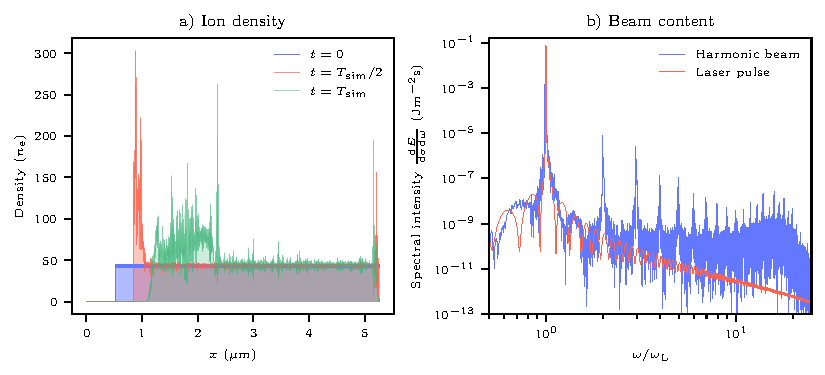
\includegraphics{figures/orion/orion_sim_figs}
	\caption[Typical 1D HHG Smilei simulation results]{\textbf{1D PIC simulation of the SP1 ORION beamline geometry at $\mathbf{a_0 = 7}$ interacting with a pre-ionised CVD target.} a) Ion density at initialisation ($t=0$), halfway ($t=T_\mathrm{sim}/2$) and at the simulation end ($t=T_\mathrm{sim}$) demonstrating hole boring. b) Absolute spectral intensity of the laser pulse and reflected harmonic beam obtained via Fourier transform. The harmonic beam retains the laser pulse spectral width. Even harmonics are significantly suppressed at this polarisation. The large bump in the distribution around the 18\th\ harmonic is spuriously generated via numerical heating.}
	\label{fig:orionsimfigs}
\end{figure}
Figure \ref{fig:orionsimfigs}a depicts ion density profile evolution via hole boring. While the density increases to several times its initial level near the plasma surface, this need not be accounted for in the hole boring calculation. Additional ions accumulating near the surface have already acquired the necessary momentum and are simply co-propagating inwards with the surface. Figure \ref{fig:orionsimfigs}b exhibits the harmonic content of the specularly reflected beam with harmonics retaining the spectral shape of the incident beam. Even harmonics are significantly suppressed relative to odd harmonics. The bump in the distribution around the 18\th\ harmonic is entirely spurious, a consequence of numerical heating. Increasing the simulation resolution shifts the bump to the right. Allowing for 10 cells per maximum harmonic wavelength, this distribution can only be trusted up to the 12\th\ harmonic. It is here the signal begins to deviate. Undoubtedly, energy conservation does not hold for this simulation. However, it is still possible to extract $I_0$. Making the reasonable assumption that Debye heating does not affect the HHG process and that the spectrum is simply the sum of the two contributions (justified by the observation of the continuation of harmonics over the bump in the distribution), $I_0$ can simply be extracted as the peak intensity of the distribution, corresponding to the intensity at $\omega/\omega_\mathrm{L}=n = 1$).

Figure \ref{fig:orioncombinedi0ds} compares the analytically calculated parameters with those extracted from the simulations. There is remarkable agreement for the parameter space accessible with the ORION laser facility and the assumptions made in the analysis.
\begin{figure}
	\centering
	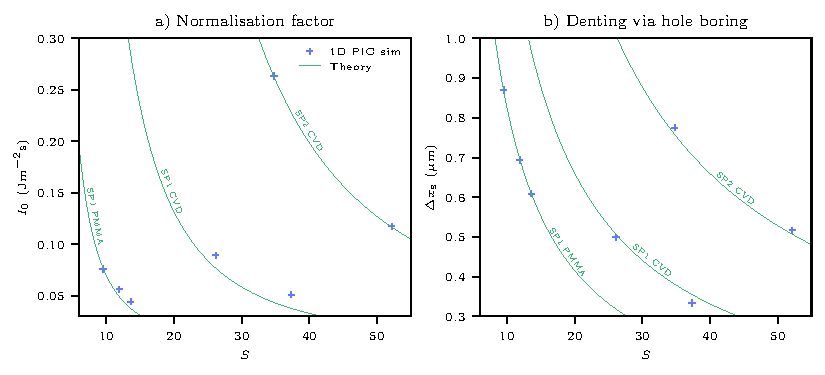
\includegraphics{figures/orion/orion_combined_I0_ds}
	\caption[Comparison between simulation and analytical predictions of hole boring and HHG normalisation factor.]{\textbf{Comparison between simulation and analytical predictions of hole boring and HHG normalisation factor in the ORION laser facility parameter space for CVD and PMMA targets.} a) The normalisation factor, $I_0$, where the spectral intensity, $I = I_0 n^{-p}$ for low order harmonics. b) The depth of hole boring compared to the initialised plasma surface. Note that the steep density gradient as visible in Figure \ref{fig:orionsimfigs}a ensures the surface position is well-defined. Both parameters are expressed in the laboratory frame.}
	\label{fig:orioncombinedi0ds}
\end{figure}
% TODO gets a new plot of above with circ pol point included. Then write following
%Note that hole boring theory relies on the assumption of a quasi-static equilibrium. This is only true for a circularly polarised incident pulse. And yet, consistent behaviour is observed for both circular and linearly polarised laser pulses.
The effect of numerical heating on the hole boring extent is illustrated by Figure \ref{fig:orioncompareiondentingtotheory} where the change in the surface position is plotted over time for the analytical calculation and PIC simulations with 2\nd\ and 4\th\ order shape function. 
\begin{figure}
	\centering
	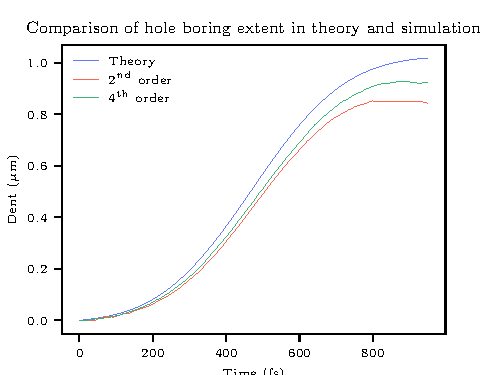
\includegraphics{figures/orion/orion_compare_ion_denting_to_theory}
	\caption[The effect of the PIC code particle shape function on numerical heating.]{\textbf{The effect of the PIC code particle shape function on numerical heating demonstrated via the extent of hole boring.} The deviation from the theoretical prediction increases with time, and the error decreases for increasing order of the shape function.}
	\label{fig:orioncompareiondentingtotheory}
\end{figure}
The deviation from the theoretical prediction increases with time. Numerical heating leads to higher electron temperatures at the plasma surface and correspondingly a spurious preplasma expansion analogous to prepulse preplasma expansion. Artificially increasing the plasma temperature to increase the Debye length and reduce numerical heating, while improving HHG accuracy\footnote{Albeit up to a point, since changes to the preplasma scale length can also affect HHG efficiency.} reduces hole boring accuracy.

The X-ray harmonic spectrum produced from a CVD target irradiated by an SP1-type laser pulse is resolved in Figure \ref{fig:orionxrayharmonics}.
\begin{figure}
	\centering
	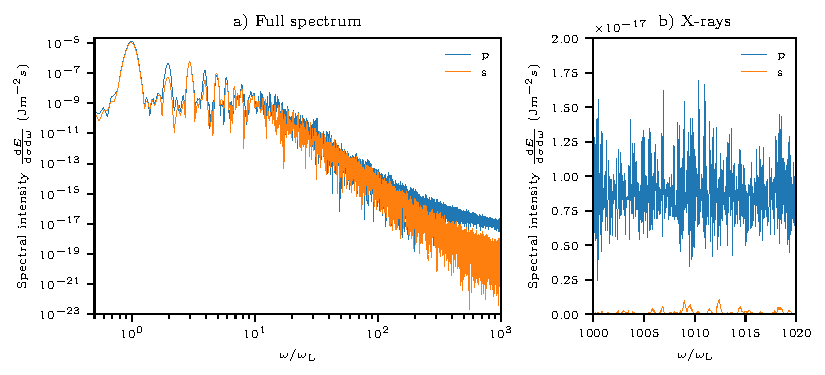
\includegraphics{figures/orion/orion_xray_harmonics}
	\caption[Reflected beam harmonic content up to the keV range in a high-resolution 1D PIC simulation.]{\textbf{Reflected beam harmonic content up to the keV range in a high-resolution 1D PIC simulation of a test pulse with SP1 ORION beam geometry incident on a CVD target.} The absolute spectral intensity is calculated from the Fourier transform of the reflected beam electric field. The s- and p-polarised components of the beam are analysed separately for both a) the full spectrum and b) the X-ray harmonics accessible with the OHREX quartz ($10\bar{1}1$) crystal.}
	\label{fig:orionxrayharmonics}
\end{figure}
The simulation has 16384 cells per laser wavelength, the minimum multiple of 2 required to resolve the harmonics accessed with the OHREX quartz crystals. It was necessary to use a short test laser pulse with a $5\lambda_\mathrm{L}$ FWHM. The simulation time before the peak of the laser pulse was increased to reduce the error in the spectrum from unphysical hard cutoffs to the laser pulse profile. A steep preplasma scale length was applied to the plasma distribution of $0.04\lambda_\mathrm{L}$ to model the peak of the ORION pulse and suppress \ac{CWE}. 
% TODO cite here the optimal length for CWE
At the X-ray intensities of Figure \ref{fig:orionxrayharmonics}b, no harmonic structure is visible, indeed for the non-optimal ORION target chamber geometry, merging begins around the 20\th harmonic. This must be accounted for in the calculation of the signal intensity. Note the s-polarised part of the reflected beam is over 50 times weaker than the p-polarised beam at the 1000\th\ harmonic.

It would be interesting to extract the reflected beam temporal profile after filtering sub-X-ray harmonics. This can be achieved by applying the inverse Fourier transform to the Fourier-transformed temporal profile with the lower-order harmonics removed. Unfortunately, beyond $n=50$, noise overwhelms the signal of interest (from ROM theory, the X-ray harmonic intensity is at least 8 orders of magnitude below the laser pulse intensity). A substantially larger simulation would be required to produce the filtered signal. Figure \ref{fig:orionattosecondpulse} compares the reflected pulse structure to the reflected pulse structure with harmonics below $n = 50$ removed. 
\begin{figure}
	\centering
	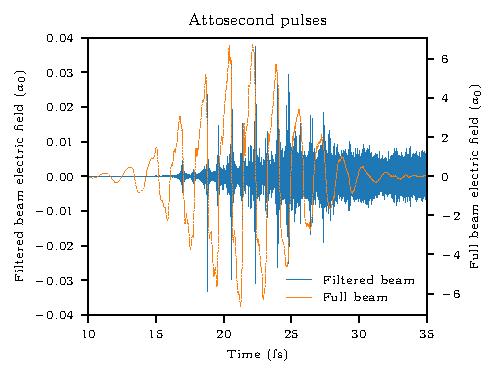
\includegraphics{figures/orion/orion_attosecond_pulse}
	\caption[Attosecond pulse train from the filtered reflected laser pulse.]{\textbf{Attosecond pulse train from the filtered reflected laser pulse.} The filtered beam contains only harmonics above $n = 50$.}
	\label{fig:orionattosecondpulse}
\end{figure}
The filtered beam consists of a series of attosecond pulses of radiation, the brightest pulse is of duration 30.3 as. This is an order of magnitude above the duration of the X-ray pulse as predicted from the cut-off expression. Note that the intensity of the first few laser cycles is insufficient for the generation of harmonics above $n = 50$ and there is therefore no signal here, effectively reducing the pulse train length.

% TODO NO Confident now that in the theory of ROM HHG for ORION parameters, there is one final consideration that cannot be observed in 1D. The SP1 beamline consists of two beamlets. Am I including this or not? For this simulation, the Bouchard solver was applied.

\subsection{Hydrodynamic simulations of preplasma formation}\ref{sec:orion-hydro}
Following Dollar \textit{et al} \cite{dollarScalingHighorderHarmonic2013}, hydrodynamic simulations of the ORION laser systems were performed using HYADES to confirm the suitability of the contrast conditions.

Simulations were performed in 1D planar geometry with a mesh of 511 evenly spaced points covering \qty{20}{\mu m} of the target (SiO2, PMMA, CVD, etc). Equation of state data was taken from the in-built HYADES data tables. For low temperatures and pressures, the data for the minimum values in the tables are used, for temperatures and pressures above the highest values recorded in the tables, the values are linearly extrapolated from this point. Ionisation was calculated using the local thermal equilibrium average atom model. Low temperature ($T < 0.15 eV$) values for the absorption and refractive indices of the target materials were input \cite{polyanskiyRefractiveindexInfoDatabase2024}.
The threshold for laser energy absorption is set to \qty{1e6}{ergs.cm^{-2}} = \qty{0.1}{W.cm^{-2}}. Electrons and ions were initialised at a temperature \qty{1.551e-2}{eV}. The real polarisation of the interaction cannot be treated using a 1D code since the electric field vector is rotated during propagation \cite{larsenQuestionSourceWave2023}. Instead, simulations were performed in both s- and p-polarisation to provide a sense of the scale of the interaction.

As expected, no pre-ionisation or preplasma formation was observed in the simulations of the high-contrast SP1 laser pulse with any target material. This is in stark contrast with the SP2 laser. In the absence of a PM, the preplasma expansion of the targets is many orders larger than the laser pulse wavelength, necessitating the use of a PM and further HYADES simulations.

The distance between the PM and the main target is \qty{15}{mm}, thus the beam diameter at the PM is $\approx 15/(f/3) = \qty{5}{mm}$. Hence, the intensity at the PM can be calculated. To account for variation around this approximation, simulations were performed with plausible high and low intensities.

First, the interaction between the SP2 beamline and a SiO$_2$ PM was simulated. Note that it is not possible to model the AR coating in hydrodynamic codes. Instead, it was assumed that the thin coating has minimal impact on the interaction. No ionisation was observed from the high-intensity laser prepulse. Figure \ref{fig:orionpmirradiation} plots the interaction between a low-intensity main pulse and the plasma mirror. 
\begin{figure}
	\centering
	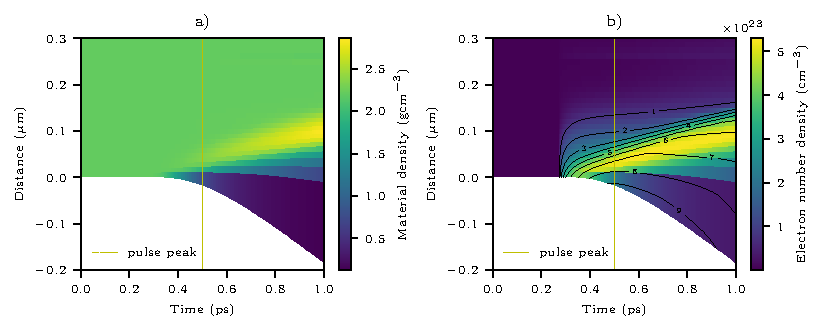
\includegraphics{figures/orion/orion_PM_irradiation}
	\caption[Silicon dioxide plasma mirror switch on from irradiation by the SP2 main pulse.]{\textbf{Silicon dioxide plasma mirror switch on from irradiation by the SP2 main pulseat \qty{45}{\degree} angle of incidence and p-polarisation.} The laser pulse travels in the $+\mathbf{\hat{x}}$-direction. The main pulse peak intensity is marked at 500 ps in the simulation. a) Material density as a function of time, a short preplasma is formed alongside hole boring. b) Electron number density as a function of time. The contours map the ionisation level.}
	\label{fig:orionpmirradiation}
\end{figure}
% TODO add a comment about at this point just getting to that ionisation threshold?
Similar results were obtained for s- and p-polarisation. These simulations suggest ionisation begins at the start of the main pulse. There is some preplasma expansion and hole boring. The focusing effect of this hole boring is minimal for the large spot size on PM and can thus be ignored. The collisionless skin depth and plasma frequency can be calculated at each mesh point in the plasma from the electron density. The corresponding laser attenuation at each point is plotted in Figure \ref{fig:orionpmreflection} at the peak of the main pulse.
\begin{figure}
	\centering
	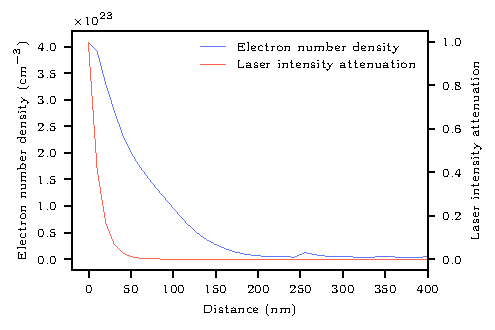
\includegraphics{figures/orion/orion_PM_reflection}
	\caption[The attenuation of the SP2 laser pulse as it propagates through a switched-on PM.]{\textbf{The attenuation of the SP2 laser pulse is calculated as it propagates through a switched-on PM.}}
	\label{fig:orionpmreflection}
\end{figure}
The laser is rapidly attenuated and therefore switched on despite not attaining total ionisation at the front surface (at a cost to its reflectivity).

Satisfied that the PM operates as anticipated, a parameter scan of the targets was then conducted. Figure \ref{fig:oriontargetpreplasma}a describes the typical evolution of target density with the application of the SP2 prepulse. In this case, the prepulse has been attenuated by a plasma mirror with a reflectivity of 0.004.
\begin{figure}
	\centering
	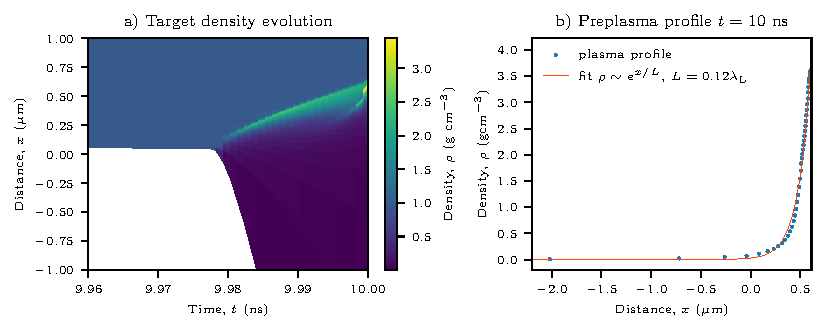
\includegraphics{figures/orion/orion_target_preplasma}
	\caption[Typical preplasma formation from the incidence of the ORION SP2 laser prepulse on a plastic target.]{\textbf{Typical preplasma formation from the p-polarised \qty{16}{\degree} angle of incidence of the ORION SP2 laser prepulse on an HDPE target.} In this simulation the laser is modelled from 10 ns before the main pulse with $a_0 = 30$ and attenuated by a PM of reflectivity 0.004. a) Typical preplasma expansion elucidated via target density. By the time of the main pulse, hole boring is dominant over plasma expansion. b) An exponetial fit ($\rho \sim e^{x/L}$) for the preplasma scale length, $L$, at the time of arrival of the main pulse. For this simulation the optimum fit is $L = 0.12 \lambda_\mathrm{L}$.}
	\label{fig:oriontargetpreplasma}
\end{figure}
By the time of the main pulse arrival in this simulation, hole boring dominates over preplasma expansion. Indeed, the laser pulse intensity has already reached relativistic intensities a couple of picoseconds out from the main interaction. Figure \ref{fig:oriontargetpreplasma}b includes an exponential fit to obtain the corresponding close to optimal preplasma scale length of $L = 0.12 \lambda_\mathrm{L}$ at the time of arrival of the SP2 main pulse.

Figure \ref{fig:orionscalelengthparameterscan} repeats the analysis of \ref{fig:oriontargetpreplasma} for a variety of target materials, reflectivities, polarisations and laser intensities.
\begin{figure}
	\centering
	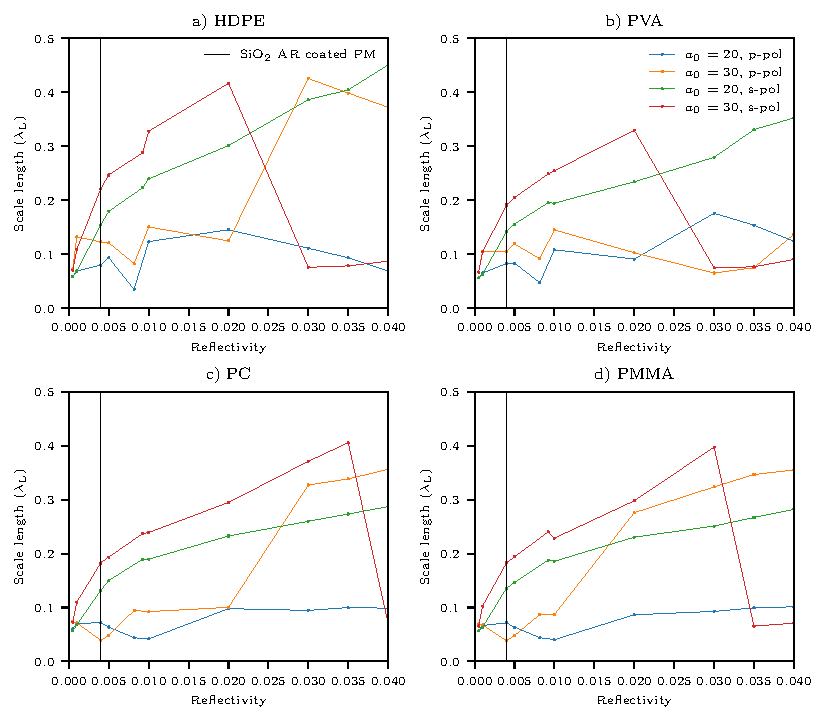
\includegraphics{figures/orion/orion_scale_length_parameter_scan}
	\caption[Preplasma scale length parameter scan.]{\textbf{Preplasma scale length parameter scan for a variety of plastic targets.} Target materials are a) HDPE, b) PVA, c) PC and d) PMMA. The dashed line highlights the reflectivity of the SiO$_2$ AR-coated PM for the SP2 wavelength. The preplasma scale length remains small for the range of parameters explored.}
	\label{fig:orionscalelengthparameterscan}
\end{figure}
The s-polarised light simulations follow a clear trend: increasing incident laser energy leads to an increased scale length up to a transition point that will be determined by the point at which hole boring overcomes plasma expansion. This will depend on the interplay of target ion density, ionisation potential and heating. Interestingly, the trend is much less consistent for p-polarised light. It is known that heating increases for p-polarised light as there is now a component of the laser pulse electric field acting into the plasma, however, the crossing of the high and low intensities suggests a dynamic balance between hole boring and plasma heating. Regardless, the change in scale length is not significant at these PM reflectivities. Unfortunately, it was not possible to conduct a similar parameter scan for the CVD targets, it would appear that the EOS tables provided for such a target material are not suited for this interaction type. However, one can assume that the preplasma scale lengths of irradiated CVD targets would be lower than those established in Figure \ref{fig:orionscalelengthparameterscan} due to the high damage threshold of the material. 

The question of plasma temperature, raised with regards to the initialisation of PIC code main pulse simulations as presented in Chapter \ref{ch:zvp}, can now be redressed. Figure \ref{fig:oriontemperature} plots the plasma electron temperature from 40 ps before the main pulse arrives.
\begin{figure}
	\centering
	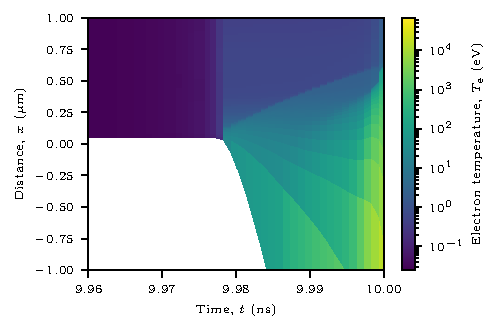
\includegraphics{figures/orion/orion_temperature}
	\caption[Typical electron temperature of a plastic target after irradiation by a petawatt class laser prepulse.]{\textbf{The typical electron temperature of a plastic target after irradiation by a petawatt class laser prepulse.} This is the same simulation as presented in Figure \ref{fig:oriontargetpreplasma}. Namely, an $a_0 = 30$ p-polarised laser pulse attenuated by a plasma mirror of reflectivity 0.004 incident on an HDPE target at \qty{16}{\degree}. The bulk and preplasma temperatures differ by multiple orders of magnitude.}
	\label{fig:oriontemperature}
\end{figure}
Once plasma expansion initiates, the extent of heating rapidly diverges across the preplasma and bulk. Evidently, it does not make sense to define a temperature for a system not in equilibrium. Indeed, there is no standardised practice within the field and yet temperature can have a significant effect, such as has already been remarked from simulations on hole boring. There is also some experimental evidence to say HHG efficiency scales inversely with plasma temperature \cite{kahalyDirectObservationDensityGradient2013}. Plasma temperature is highly sensitive to the precise experimental conditions. At the time of the main pulse arrival at the plasma surface (as defined by the peak of the electron density distribution), the temperature is 112 eV. This is at least consistent with the value chosen for PIC simulations but should be treated with wariness. 

Note hydrodynamic codes would be unsuitable for the prediction of the plasma temperature increases induced by the main pulse interaction given the high non-linearity of the dynamics in this regime that could not be adequately captured by such a code.

% TODO in the intro explains the local thermal equilibrium average atom model for ionisation.

\section{\label{ch:3-sec:experiment}The experiment}
The two experimental goals were to resolve and measure the absolute intensity of X-ray harmonics produced by the interaction of the ORION SP2 beamline with a range of flat solid targets. After debris from the plasma mirror optic damaged the parabola it was necessary to switch to the higher contrast but lower energy SP1 beamline. Only after the experiment was it established from simulations that it is not possible to resolve X-ray harmonics with the ORION target chamber geometry. However, absolute intensities were measured for both the SP1 and SP2 beamlines and for CVD and PMMA targets. ORION short pulse beamline parameters are provided in Figure \ref{tab:laser_params}.

The experimental design is relatively straightforward. CAD drawings of the experimental setup are presented in Figure \ref{fig:orioncad}.
\begin{figure}
	\centering
	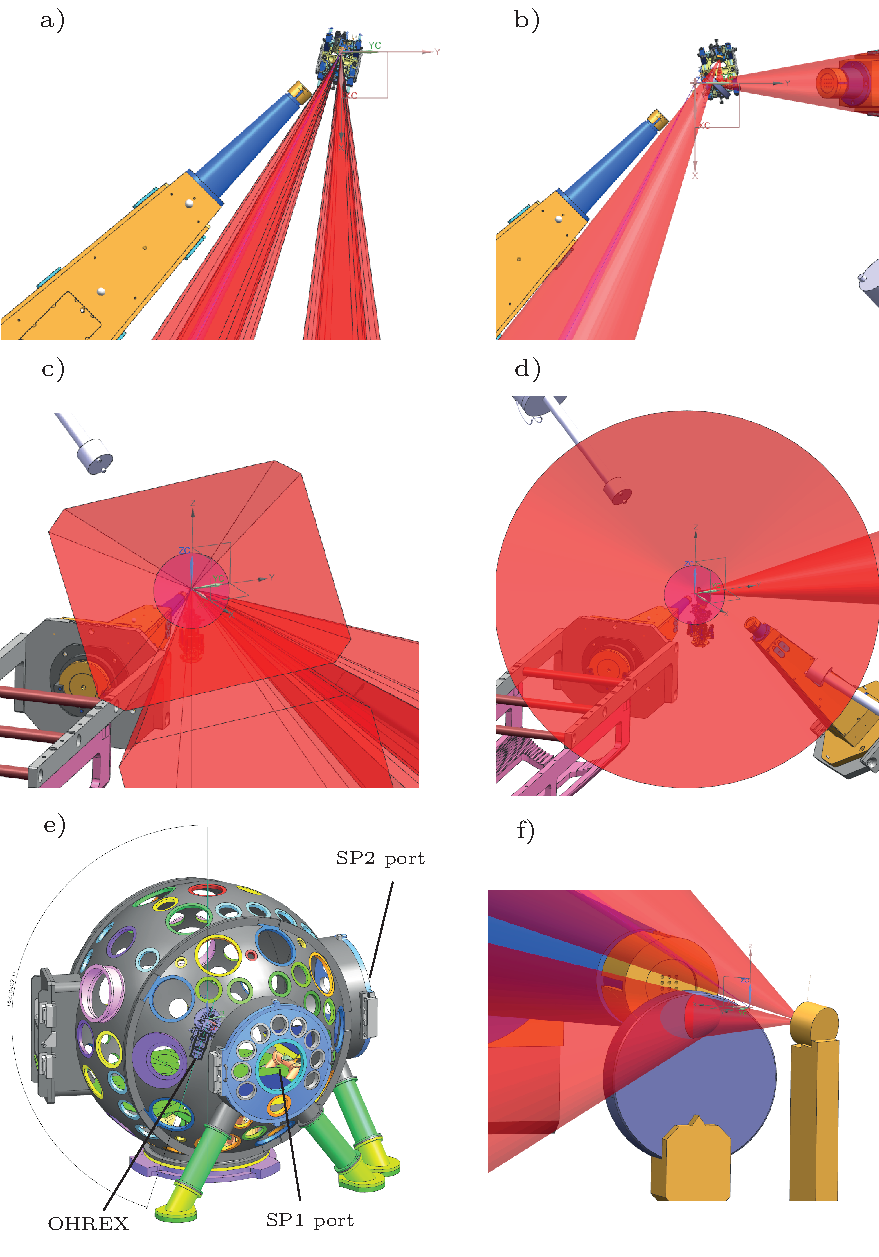
\includegraphics[width=1\linewidth]{figures/orion/orion_cad}
	\caption[ORION HHG experiment target chamber set up.]{\textbf{CAD images of the ORION target chamber set up for this experiment.} a) and b) SP1 and SP2 beamlines respectively from parabola to TCC to OHREX spectrometer. c) and d) SP1 and SP2 beamlines respectively looking from OHREX to TCC. e) Annotated ORION target chamber model. f) SP2 beamline reflecting off plasma mirror before main target incidence.}
	\label{fig:orioncad}
\end{figure}
The laser was focused onto the target at \ac{TCC} with the \ac{OHREX} spectrometer positioned along the specular reflection direction. Additional X-ray pinhole diagnostics monitored the spot size. The SP2 beamline reflects off an additional \ac{PM} optic at \qty{45}{\degree} \ac{AOI} before the main target to improve the laser prepulse contrast. Then both the SP1 and SP2 beamlines arrive at \ac{TCC} along the same axis.

\subsection{Target chamber geometry and polarisation}
Both the non-linear HHG interaction and the linear OHREX crystal spectrometer are sensitive to the polarisation of incident light. It is therefore important to track the polarisations of the beamlines as they propagate through the system.

The ORION target chamber has its own defined geometry with the target located at the origin (\ac{TCC}), sketched in Figure \ref{fig:miscoriontargetchambergeometry}.
\begin{figure}
	\centering
	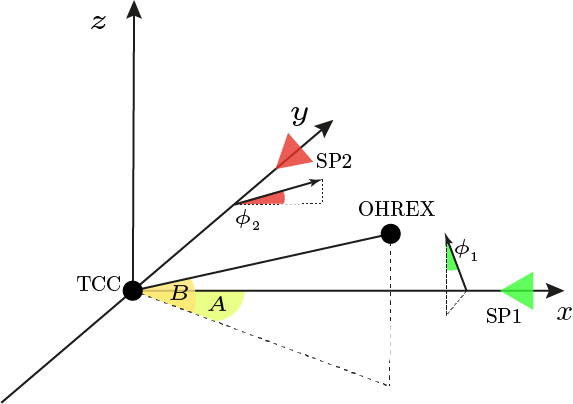
\includegraphics[width=0.7\linewidth]{figures/misc/misc_ORION_target_chamber_geometry}
	\caption[ORION target chamber geometry]{ORION target chamber geometry with the location of the target, OHREX spectrometer and the SP1 (green) and SP2 (infra-red) beamlines and their corresponding polarisations, $\phi_1$ = \qty{11.8}{\degree} and $\phi_2$ = \qty{16.4}{\degree}.}
	\label{fig:miscoriontargetchambergeometry}
\end{figure}
The polarisation angles of the two beamlines are $\phi_1 = \qty{11.8}{\degree}$ and $\phi_2 = \qty{16.4}{\degree}$. Following the reflection of the SP2 beam off the plasma mirror, both the SP1 and SP2 beamlines propagate in the -$\hat{\mathbf{x}}$-direction towards the origin. The OHREX crystal is located at 
\begin{equation}
	\mathbf{r}_\mathrm{OHREX} = r_0(\cos B\cos A,-\cos B\sin A, \sin B),
\end{equation}
where $r_0 = \qty{2.4}{m}$, $A = \qty{26.82} {\degree} $ and $B = \qty{18.15}{\degree}$, setting the rotation angle of the target. As in Figure \ref{fig:orioncad}e, the OHREX spectrometer sits on the outside of the target chamber tilted an angle \qty{18}{\degree} to the vertical.

The interaction plane is defined by the vector
\begin{equation}
	\mathbf{n} = \frac{\mathbf{r}_\mathrm{OHREX}}{r_0} \times  \hat{\mathbf{x}} = (0,\sin B, \cos B\sin A).
\end{equation}
The cosine rule can be applied to determine the polarisation of the laser pulses in the interaction plane, for polarisation vector $\hat{\mathbf{E}}$,
\begin{equation}
	\frac{\mathbf{n}}{|\mathbf{n}|}\cdot\hat{\mathbf{E}} = \cos\theta,
\end{equation}
where $\theta$ defines the angle between the polarisation vector and the vector normal to the interaction plane. This corresponds to angles out of the interaction plane of \qty{42.2}{\degree} for the SP1 beam (rotating anticlockwise out of the interaction plane when looking from TCC to parabola) and \qty{19.6}{\degree} for the SP2 beam (rotating clockwise out of the interaction plane when looking from TCC to parabola). Again applying the cosine rule, the angle of incidence is \qty{16}{\degree}.

The polarisation vector can then be split into s- and p-polarised components. The s-polarised component remains unchanged by the interaction but the p-polarised component must be rotated, its direction along $\mathbf{n} \times \mathbf{r}_\mathrm{OHREX}$. Figure \ref{fig:orionxrayharmonics} illustrates the suppression of the s-polarised component at the X-ray photon energies of interest. This component is therefore neglected.

The OHREX spectrometer sits flat on the target chamber wall but rotated an angle $C= $ \qty{18}{\degree} to the vertical. The OHREX interaction plane is correspondingly rotated. Again, applying the cross-product, the OHREX interaction plane is 
\begin{equation}
	\mathbf{n}_\mathrm{O} = [-\cos(A)\sin(B)\sin(C)-\sin(A)\cos(B)\cos(C),-\cos(A)\cos(B)\cos(C)+\sin(A)\sin(B)\sin(C),\cos(B)\sin(C)].
\end{equation}
Applying the cosine rule between the p-polarised vector and $\mathbf{n}_\mathrm{O}$, the angle of the polarisation vector of the harmonic beam out of the plane of the OHREX interaction is \qty{77.23}{\degree} for both SP1 and SP2.

\subsection{Targets}
Specialised target holders were designed and built by the AWE and CLF target fabrication teams. These hold the targets at the required angle out of the horizontal plane with an additional fiducial wire for alignment. Targets were mounted on the ORION Multi-Target-Mount and alignment was performed offline by Dr Ed Gumbrell.

There are multiple considerations when it comes to target density. In practice accessing the $S\approx 1$ regime is not possible using a petawatt class laser system with even the lowest density solid plastic targets. However, the 2007 Vulcan experiment successfully reproduced the $8/3$ scaling up to the X-ray regime for $S \approx 50 $ \cite{dromeyBrightMultikeVHarmonic2007} despite simulations repeatedly emphasising the improvement of harmonic efficiency for reduced similarity parameter. At the same time, as discussed in Section \ref{ch:3-sec:theory}, target hole boring leads to an increased harmonic beam divergence. High electron density targets are perhaps therefore more suited to the petawatt class laser system thereby maintaining the beaming of harmonics.
% TODO finds that paper where they show that CSE lowers the roll-off point, I did read this somewhere...
% Vulcan had CH targets, a0 on target of approx 6.2, normalised density approx 308.
%TODO comment on improvement of S parameter for PMMA leading to an increase in signal strength?

% TODO use the word perturbation for surface roughness
The surface perturbation of a selection of low-density plastic targets was analysed by the CLF target fabrication team leading to the choice of PMMA plastic targets. CVD targets were also selected, having the highest ionisation potential (and therefore lowest susceptibility to laser prepulse) of solids that can be polished optically flat albeit at a higher $S$ parameter. Target surface scans performed by AWE and CLF are given in Figure \ref{fig:oriontargets} \cite{spindloePlasticTargetsOrion2023}.
\begin{figure}
	\centering
	%\includegraphics{figures/orion/orion_targets}
	\caption[ORION HHG experiment targets]{\textbf{ORION experiment 3D scans of target roughness.} a) CVD with roughness $\Delta s$ = \qty{4}{nm} and $S \approx$ 26, 35 for SP1 and SP2 beamlines respectively. b) PMMA with roughness $\Delta s$ = \qty{11.2}{nm} and $S \approx$ 10, 13 for SP1 and SP2 beamlines respectively.}
	\label{fig:oriontargets}
\end{figure}

\subsection{Contrast and plasma mirrors}
As illustrated in Figure \ref{fig:orioncad}, a plasma mirror optic is included before the main target to improve the contrast of the SP2 beamline \cite{doumyCompleteCharacterizationPlasma2004}. HYADES simulations of the effect of this optic are detailed in Section \ref{sec:orion-hydro}. Provided the harmonic beam divergence is less than or equal to the $f/3$ cone of the laser pulse, as is anticipated, the harmonic beam should not be clipped by the PM in this setup. 

The intention was to use \ac{AR}-coated fused silica optimised for \qty{45}{\degree} \ac{AOI} and the SP2 pulse wavelength (BCP45R) \cite{45AOIBeamsplitter}. This has a reflectance of \qty{0.398}{\%} at $\lambda_\mathrm{L} = \qty{1053}{nm}$ for unpolarised light. Unfortunately, the debris from the PM caused damage to the parabola. For the second SP2 shot, the high reflectivity fused silica PM was replaced by a thin foil of silicon nitride. The reduction in available material of the thin foil lowers the risk of damaging debris. At \qty{45}{\degree} \ac{AOI}, $\lambda = \qty{1.053}{\mu m}$ and $\phi_2 = \qty{16.4}{\degree}$, the silicon nitride PM pre-switch-on has a reflectivity of \qty{5.55}{\%} \cite{polyanskiyRefractiveindexInfoDatabase2024}. It is safe to assume consistent behaviour after switch-on for the two PMs.

\section{\label{ch:3-sec:data_processing}Experimental data processing}
\subsection{Image plate calibration}
Image plates (IPs) are reusable recording media that detect ionising radiation and are particularly suitable for the detection of X-rays produced in laser-plasma interactions. Their response is well understood and their sensitivities to a wide spectrum of photon energies have been absolutely calibrated on the ORION facility \cite{meadowcroftEvaluationSensitivityFading2008}, albeit for the FLA3000 scanner, not the FLA7000 used in this experiment. However, the deviation in response is negligible for the photon energies measured. In this experiment, the Fuji Biological Analysis System (BAS) TR-type IPs were used. They have a phosphor layer composed of $\mathrm{BaFBr_{0.085}I_{0.15}}$ with density \qty{2.61}{g.cm^{-3}} and thickness \qty{60}{\mu m} but no mylar layer. This makes them suitable for low-energy X-ray detection. When scanned, the IP releases blue photons via photostimulated luminescence (PSL), which are then collected by a photomultiplier tube. The PSL value is generalised across scanner types from the measured `Grey' ($G$) value by
\begin{equation}
	\mathrm{PSL} = (0.23284G^2\times 10^{-9})\left(\frac{\Delta x}{100}\right)^2W\times 10^{-L/2},
\end{equation}
where $\Delta x$ is the scanner resolution (= \qty{25}{\mu m} in this experiment), $L$ is the latitude parameter, and
\begin{equation}
	W = 0.092906 + 1370.8e^{-0.014874V} +  654.24e^{-0.011026},
\end{equation}
where $V$ is the scanner voltage \cite{golovinCalibrationImagingPlates2021}.

IP photon sensitivity, $\psi$, the number of PSLs per incident photon, is dependent on photon energy. Meadowcroft \textit{et al} modelled this as,
\begin{equation}
	\psi_j = \eta(m_jh\nu + c_j),
\end{equation}
where $h\nu$ is the photon energy and $m_j$ and $c_j$ are linear fit parameters valid for specific energy ranges, $j$. For the Fuji BAS TR-type IP and X-rays in the range 0-6.0 keV, $m_j = \qty{0.54\pm0.05}{mPSL.keV^{-1}}$ and $c_j = \qty{0.02\pm0.002}{mPSL}$. The IP absorption efficiency in mPSL per photon is
\begin{equation}
	\eta(h\nu,T_i,T_s) = \exp{(-n_\mathrm{i}\Phi_\mathrm{i} (h\nu)T_\mathrm{i})}[1-\exp{(-n_\mathrm{s}\Phi_\mathrm{s}(h\nu)T_\mathrm{s})}],
\end{equation}
where $n$ is the layer density, $\Phi(h\nu)$ is the total cross-section of the layer, $T$ the effective layer thickness, s and i correspond to the sensitive (phosphor) and insensitive (mylar) layers of the IP respectively \cite{izumiApplicationImagingPlates2006}. The first term is neglected in the absence of an insensitive (mylar) layer in TR-type IP. Below 50 keV, the dominant mode for X-ray absorption into the IP is the photo-electric effect, where
\begin{equation}
	\Phi_\mathrm{ph} \approx \num{3e12}\frac{Z^4}{(h\nu)^{3.5}}   
\end{equation}
and $Z$ is the atomic number \cite{fornalskiSimpleEmpiricalCorrection2018} and $\Phi_\mathrm{ph}$ is given in units of Barn per atom. At 2.4 keV, that corresponds to a sensitivity of 1.32 mPSL per incident photon.

It is generally unavoidable that some time will elapse between the laser shot and the IP scan. For this experiment, 30 minutes was typical, in which time some fading of the IP occurs that must be accounted for. IP fading can be modelled as an attenuation factor,
\begin{equation}\label{eq:orion.Ft}
	F(t) = A\exp{(-t/\tau)} + B,
\end{equation}
where $t$ is the time between shot and scan and $A$, $\tau$ and $B$ are found from fits to experimental data. A key aspect of the exponential decay is that the attenuation depends only on the signal at that moment in time and not the initial conditions. This has been shown to be true in experiment \cite{meadowcroftEvaluationSensitivityFading2008}.

At \qty{20}{\degree C} at the ORION facility, \textit{Meadowcroft et al} \cite{meadowcroftEvaluationSensitivityFading2008} determined that for the Fuji BAS TR-type IP, the optimum fit for the parameters of Equation \ref{eq:orion.Ft} is $A = \num{0.347\pm0.022}$, $B = \num{0.693\pm0.011}$ and $\tau = \qty{35.5\pm5.3}{minutes}$. Therefore at 30 minutes, $F(t) = 0.84$.

In summary, the number of PSL measured on an IP can be converted to an incident number of photons via
\begin{equation}
	N(h\nu) = \frac{\mathrm{PSL}}{F(t)}\frac{10^3}{\psi(h\nu)} = P(h\nu) \mathrm{PSL}.
\end{equation}

\subsection{OHREX calibration}
The Orion High REsolution X-ray (OHREX) spectrometer, housed on the ORION laser target chamber outer wall, utilises a spherically bent crystal geometry to spatially focus and spectrally analyse photons from the target chamber \cite{beiersdorferLineshapeSpectroscopyVery2016} with a high signal-to-noise ratio. The measured signal has been absolutely calibrated for a range of X-ray photon energies using a variety of crystals \cite{macdonaldAbsoluteThroughputCalibration2021}. The OHREX spectrometer can hold two crystals at a time. At each crystal's spatial focal plane, a two-dimensional image is formed, one dimension is spatial, the other spectral. The energy range accessed by a given crystal is determined by the crystal rotation but all OHREX crystals are designed for operation at a nominal central Bragg angle of $\theta_\mathrm{B} = 51.3$\degree with the corresponding wavelength determined from Bragg's Law, $n\lambda = 2d\sin\theta_\mathrm{B}$, for the appropriate crystal plane. The range around that central photon energy is determined by the crystal width in the spectral dimension.

MacDonald \textit{et al} determined a quadratic fit for each crystal's dispersion relation to connect position along the crystal image to photon energy \cite{macdonaldAbsoluteThroughputCalibration2021}. Unfortunately in this experiment, the image lengths varied from those in the previous experiment, a likely consequence of slight defocusing of the optic. The OHREX geometry is designed such that precise focus is not necessary to achieve good results and optimisation is not routinely performed \cite{beiersdorferLineshapeSpectroscopyVery2016}.

Instead, a simple linear dispersion relation based on the known maximum and minimum energies accessed by the crystal was applied across the crystal images, a reasonable approximation to the dispersion relation determined by MacDonald \textit{et al} \cite{macdonaldAbsoluteThroughputCalibration2021} (the quadratic correction is small). The energy ranges for the three lowest energy OHREX crystals are given in Table \ref{tab:dispersion}.
\begin{table}
	\centering
	\begin{tabular}{ccc}
		\hline \hline
		Crystal               & Range, $n=1$ (eV) & Range, $n=2$ (eV) \\ \hline
		KAP (100)             & 585-625          & 1170-1245        \\
		Quartz ($10\bar{1}0$) & 1830-1950        & 3660-3900        \\
		Quartz ($10\bar{1}1$) & 2330-2480        & 4660-4960  \\     \hline \hline
	\end{tabular}
	\caption{\label{tab:dispersion} Photon energy ranges captured by the three lowest energy OHREX crystals when operating at their nominal central Bragg angle of 51.3\degree for first and second diffraction orders, $n$.}
\end{table}

Provided full illumination of the \qty{6}{cm} $\times$ \qty{4}{cm} crystal, as can be assured for harmonic beams at 2.4 m from the target, the spatial dimension can be safely integrated over to calculate the measured signal, $M(h\nu)$ in \unit{J.mm^{-1}} and remove uncertainty from the IP drifting from the ideal focal plane.
% (In this experiment we assume that the harmonic beam width at the crystal position is larger than the size of the crystal, a reasonable assumption since beam divergence $\approx$ \qty{10}{\degree} and the \qty{6}{cm} x \qty{4}{cm} crystal sits \qty{2.4}{m} from the target.). 
This corresponds to a source spectral intensity incident on the crystal $S(h\nu)$ measured in \unit{J.keV^{-1}.sr^{-1}} via the spectrometer response, $G(h\nu)$, explicitly,
\begin{equation}
	M(h\nu) = S(h\nu)G(h\nu).
\end{equation}
The absolute throughput of the crystals was measured by MacDonald \textit{et al} in a previous ORION experiment and fit parameters for 
\begin{equation}
	G(h\nu) = A(h\nu)^2 + B(h\nu) + C,
\end{equation}
where $(h\nu)$ is the photon energy measured in eV, were determined for both p- and s-polarised incident light and for first and second diffraction orders \cite{macdonaldAbsoluteThroughputCalibration2021}. The parameters for the lowest few energy crystals are presented in Table \ref{tab:orion_OHREX}.
\begin{table}
	\centering
	\begin{tabular}{cccccc}
		\hline \hline
		Crystal               & Order & Polarisation & $A$            & $B$             & $C$            \\
		\hline
		KAP             & 1     & s            & \num{1.72e-15} & \num{-4.69e-12} & \num{2.89e-9}  \\
		(100) &       & p            & \num{1.40e-14} & \num{-1.74e-11} & \num{5.42e-9}  \\
		& 2     & s            & \num{3.64e-16} & \num{-9.64e-13} & \num{6.95e-10} \\
		&       & p            & \num{5.03e-10} & \num{8.09e-13}  & \num{5.03e-10} \\
		Quartz  & 1     & s            & $\cdots$       & $\cdots$        & $\cdots$       \\
		($10\bar{1}0$)&     & p            & $\cdots$       & $\cdots$        & $\cdots$       \\
		& 2     & s            & \num{4.50e-15} & \num{-3.40e-11} & \num{6.52e-8}  \\
		&       & p            & \num{1.13e-15} & \num{-8.86e-12} & \num{1.73e-8}  \\
		Quartz  & 1     & s            & \num{1.00e-16} & \num{-1.74e-12} & \num{4.93e-9}  \\
		($10\bar{1}1$)&     & p            & \num{2.78e-15} & \num{-1.41e-11} & \num{1.79e-8}  \\
		& 2     & s            & \num{4.70e-16} & \num{-4.50e-12} & \num{1.11e-8}  \\
		&       & p            & \num{2.10e-16} & \num{2.11e-12}  & \num{5.30e-9}  \\
		\hline \hline
	\end{tabular}
	\caption{Sensitivity fit parameters as a function of photon energy, $h\nu$ in electron-volts ($G(h\nu) = A(h\nu)^2 + B(h\nu) + C$) for the three lowest energy OHREX crystals for p- and s-polarised incident photons and first and second diffraction orders \cite{macdonaldAbsoluteThroughputCalibration2021}. Note that no data is available for the first order of the quartz ($10\bar{1}0$) crystal.}
	\label{tab:orion_OHREX}
\end{table}
There is unfortunately no spectrometer response data for the $10\bar{1}0$ crystal to first order due to the Si K edge within that energy range and the dramatic effect this has on absorption in its vicinity \cite{hellCalibrationOHREXHighresolution2016}.

The OHREX is equipped with a \qty{50}{\mu m} Beryllium filter to protect the crystals. The corresponding signal attenuation can be calculated using X-ray transmission data \cite{henkeXRayInteractionsPhotoabsorption1993}.

\subsection{Extracting the data}
The quartz OHREX crystals $10\bar{1}0$ and $10\bar{1}1$ were fielded on the experiment. Crystal images were recorded with BasTR2040 Fuji Image Plate. A typical shot image scanned with the FLA7000 scanner and converted to photostimulated luminescence units (PSLs) is presented in Figure \ref{fig:orionohrexshot28psl}.
\begin{figure}
	\centering
	\includegraphics[width=0.5\linewidth]{figures/orion/orion_OHREX_shot28_psl}
	\caption[Unprocessed IP from ORION experiment]{Unprocessed shot data from a FLA7000 scanned image plate converted to PSLs. The image plate and two crystal images are clearly visible.}
	\label{fig:orionohrexshot28psl}
\end{figure}
The average background signal was subtracted. The $x$- and $y$-axes were converted from pixels to mm using the scanner resolution, (\qty{25}{\mu m.px^{-1}}), and then to photon energies using the appropriate dispersion relations. The data was integrated over $y$ to obtain the intensity in units of \unit{PSL.mm^{-1}} across each crystal image. The corresponding source signal is thus
\begin{equation}
	S(h\nu)[\unit{J.keV^{-1}.sr^{-1}}] = \frac{d\mathrm{PSL}}{dx}\frac{P(h\nu)}{G(h\nu)}h\nu,
\end{equation}
which can then be converted to a measured spectral intensity per harmonic per steradian, ready to be directly compared to the theory,
\begin{equation}
	I^\mathrm{meas}_\mathrm{n}|_{(r = \qty{1}{m})} = S(h\nu)\frac{dh\nu(keV)}{dn}.
\end{equation}

No sensitivity data is available for the $10\bar{1}0$ quartz crystal, instead, this lower energy crystal was fielded to attempt resolving of the X-ray harmonics. Figure \ref{fig:orionq1010} is a typical integrated signal in \unit{PSL.mm} and the corresponding Fourier transform for the quartz ($10\bar{1}0$) crystal image.
\begin{figure}
	\centering
	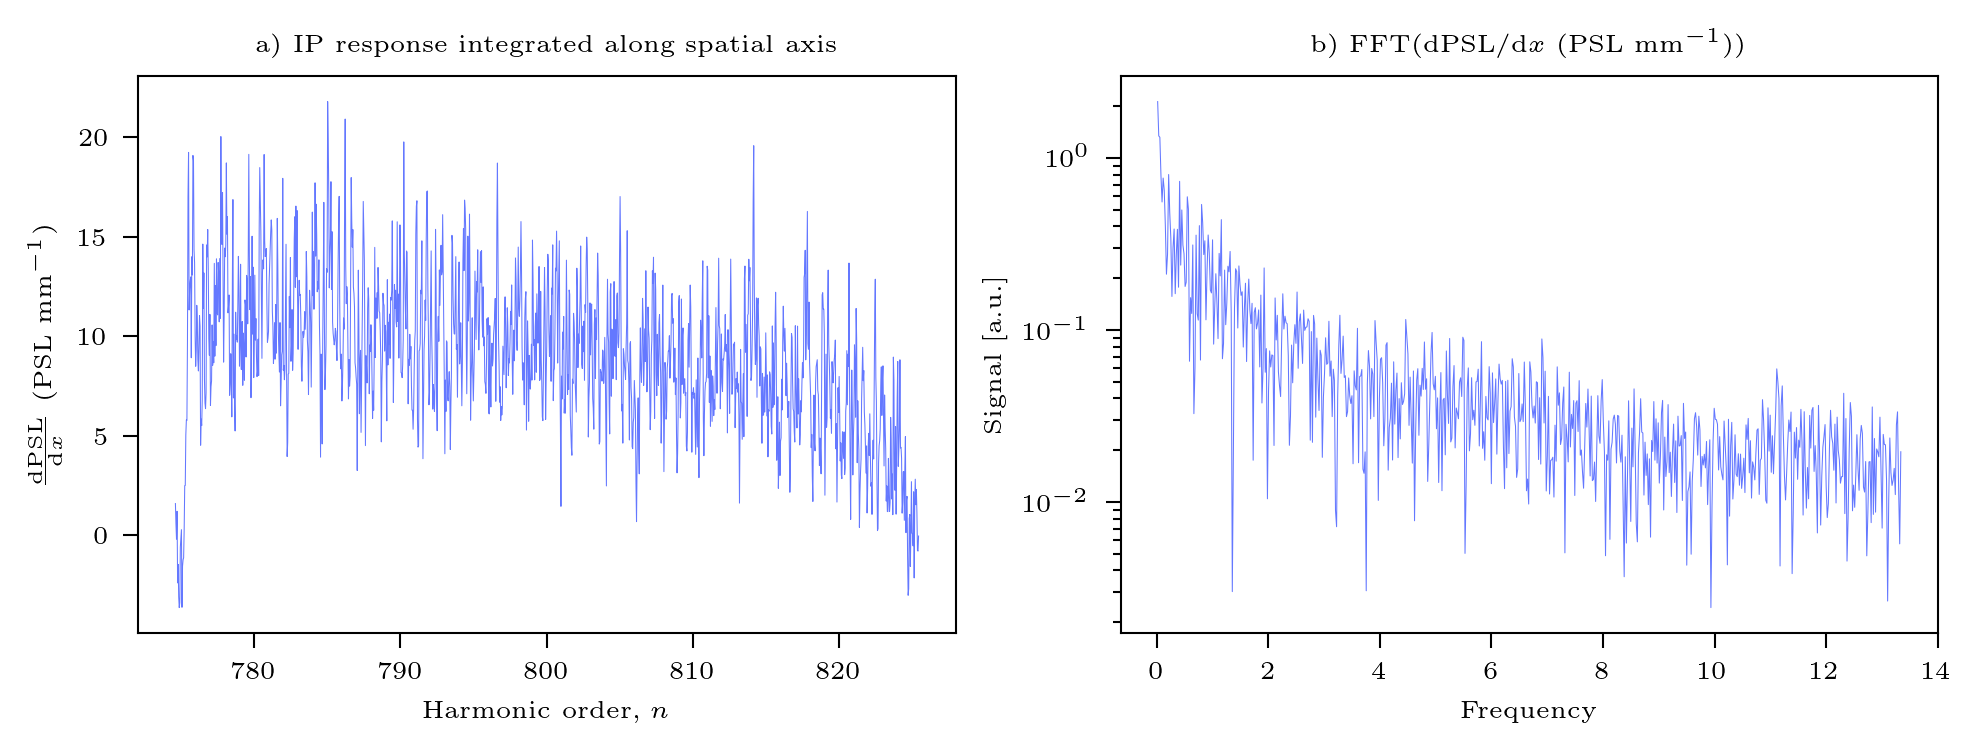
\includegraphics[width=1\linewidth]{figures/orion/orion_q1010}
	\caption[Typical ORION experiment uncalibrated IP response quartz ($10\bar{1}0$) crystal and Fourier transform]{\textbf{Typical (SP1, PMMA) uncalibrated shot data for the quartz ($10\bar{1}0$) image} a) IP spatial axis integrated signal with dispersion axis. b) Fourier transform of a) with no evidence of harmonics.}
	\label{fig:orionq1010}
\end{figure}
As anticipated harmonics cannot be resolved.

\subsubsection{Calibration and polarisation}
The choice of the spectrometer response function, $G(h\nu)$, is non-trivial. One must first be assured that the second-order contribution is small relative to the first, true for this source spectrum. And also think carefully about the anticipated polarisation in the OHREX interaction plane. The OHREX response to p-polarised light is approximately an order of magnitude lower than for s-polarised light. The polarisation of the HHG beam relative to the OHREX plane of incidence and reflection is \qty{10.5}{\degree} out of the plane. Unlike the RPM interaction, the OHREX crystal reflection is an entirely linear process and it is therefore acceptable to decompose the laser pulse into its constituents, explicitly, the field incident on the crystal is
\begin{equation}
	\mathbf{E_\mathrm{O}} = \mathbf{E}_\mathrm{O,\, s} + \mathbf{E}_\mathrm{O,\, p}.
\end{equation}
After interaction with the crystal, the field is
\begin{equation}
	\mathbf{E}_\mathrm{detector} = \alpha_\mathrm{s}(h\nu)\mathbf{E}_\mathrm{O,\, s} + \alpha_\mathrm{p}(h\nu)\mathbf{E}_\mathrm{O,\, p},
\end{equation}
where $\alpha_i(h\nu)$ is the energy-dependent $(h\nu)$ amplitude sensitivity of the reflection for s- and p-polarised respectively. Since the two polarisations are orthogonal, the intensity is
\begin{equation}
	I = \alpha^2_\mathrm{s}(h\nu)|\mathbf{E}_\mathrm{O,\, s}|^2 + \alpha^2_\mathrm{p}(h\nu)|\mathbf{E}_\mathrm{O,\, p}|^2.
\end{equation}
Noting that $\alpha^2_i(h\nu)$ are the calibration factors, $G_i(h\nu)$, and that
\begin{equation}
	|\mathbf{E}_\mathrm{O,\, s}| = |\mathbf{E_\mathrm{O}}|\sin\phi
\end{equation}
and
\begin{equation}
	|\mathbf{E}_\mathrm{O,\, p}| = |\mathbf{E_\mathrm{O}}|\cos\phi,
\end{equation}
where $\phi$ is the angle out of the interaction plane,
\begin{equation}
	I_\mathrm{detector} = (G_\mathrm{s}(h\nu)\sin^2\phi + G_\mathrm{p}(h\nu)\cos^2\phi)|\mathbf{E_\mathrm{O}}|^2 = F(h\nu)|\mathbf{E_\mathrm{O}}|^2,
\end{equation}
where $F(h\nu) =  (G_\mathrm{s}(h\nu)\sin^2\phi + G_\mathrm{p}(h\nu)\cos^2\phi$ is the energy-dependent calibration factor for this OHREX orientation.

\subsection{KBRXM}
The ORION SP1 and SP2 spot size was routinely monitored on shot by the AWE laser team via two X-ray pinhole cameras and the time-integrating Kirkpatrick-Baez X-ray microscope (KBXRM) diagnostic, sat on the target chamber Port 21 and pointed at the notional \ac{TCC}. This reflective X-ray microscope optic has a ten times magnification and spatial resolution of \qty{15}{\mu m}, comfortably resolving the laser spot size. Images were again recorded with TR-type IP. Direct mapping between the recorded images and real laser irradiance profiles is a highly non-trivial problem with any proposed model depending strongly on the assumptions made. However, by making the very reasonable assumption of spatial and temporal blurring of the spot size in the X-ray image due to electron transport away from the laser spot, the measured spot size will be an upper bound on the real spot size. It follows that the upper bound on optical spot widths corresponds to a lower limit of irradiance (since the on-shot energy is well-defined). These diagnostics determine sensible upper bounds for the laser spot size are \qty{20}{\mu m} and \qty{10}{\mu m} for the SP1 and SP2 beamlines respectively.

\section{\label{ch:3-sec:results}Experimental results}
Figure \ref{fig:orionq1011} is a typical calibrated signal from the quartz ($10\bar{1}1$) crystal, ready for comparison to the theoretical prediction.
\begin{figure}
	\centering
	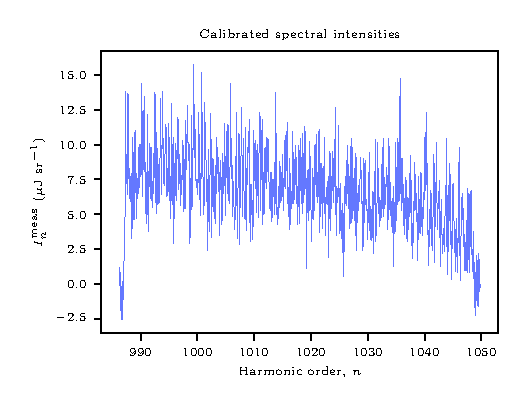
\includegraphics[width=0.7\linewidth]{figures/orion/orion_q1011}
	\caption[Typical ORION experiment calibrated IP response for the quartz ($10\bar{1}1$) crystal.]{Typical (SP1, PMMA) ORION experiment calibrated IP response for the quartz ($10\bar{1}1$) crystal.}
	\label{fig:orionq1011}
\end{figure}
For each shot the mean signal across the dispersion axis was calculated and the errors from statistics, the fade time (11 \%), the IP sensitivity (1.5 \%), the dispersion axis (2.9 \%) and the OHREX crystal reflectivity (11 \%) accounted for.

As demonstrated in Section \ref{ch:3-sec:theory}, the intensity of X-ray harmonics is highly sensitive to the intensity of individual pulse cycles due to the proximity of the measurement to the exponential roll-off in the spectrum. However, even neglecting the shot-to-shot variation, it is not possible to know the precise sub-cycle spatio-temporal structure of a petawatt-class laser pulse. Indeed, the simple measurement of the peak intensity of such a pulse remains an open problem \cite{perevalovLaserPeelerRegime2023,ouatuIonizationStatesMultipetawatt2022}. Approximations and assumptions must be made, that is, that the SP1 and SP2 beamlines can be adequately described by spatial Gaussians and temporal sech$^2$ and sech profiles respectively, and that the duration and energy are well-defined. 

The upper limit on laser pulse spot size obtained from the KBRXM diagnostic corresponds to a lower limit on laser pulse intensity and therefore also of XHHG efficiency near roll-off. Figure \ref{fig:orionintensitycurves} plots XHHG spectral intensity curves for the quartz ($10\bar{1}1$) crystal central energy as a function of laser spot size for the targets and laser pulse configurations explored in the experiment. 
\begin{figure}
	\centering
	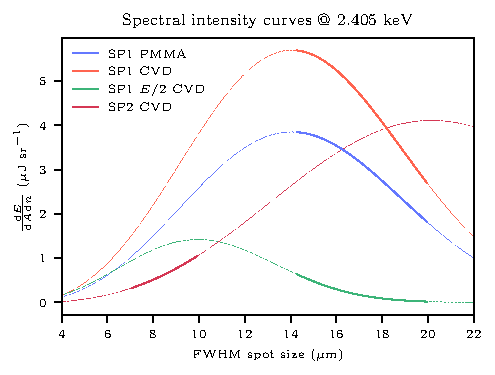
\includegraphics{figures/orion/orion_intensity_curves}
	\caption[Dependence of the harmonic beam spectral intensity on laser spot size at 2.405 keV.]{\textbf{Dependence of the harmonic beam spectral intensity on laser spot size at 2.405 keV.} Targets and beamlines relevant to the experiment are plotted. The half-energy single beamlet SP1 laser is demarcated by $E/2$. The thick lines indicate likely values for the laser spot sizes in this experiment. The SP1 harmonic beams are strongly affected by the exponential roll-off, unlike the SP2 beamline.}
	\label{fig:orionintensitycurves}
\end{figure}
The thick lines range from the upper limits of spot size as measured by the KBRXM diagnostic to a spot area half that for the upper bound, a reasonable lower bound on the spot size. The spectral intensity of the harmonic beam from the SP1 beamline sits in a delicate balance between beam divergence via hole boring and the exponential roll-off. Note that only the roll-off leads to a reduction in the total energy contained within the harmonic beam. The strong non-linearity of the interaction leads to the single beamlet SP1 beamline producing a harmonic beam over 6 times weaker than the double beamlet configuration. Interestingly, the higher intensity of the SP2 beamline causes greater divergence and a lower spectral intensity of the harmonic beam than for the SP1 laser pulse.

Figure \ref{fig:orionexperimentresults} plots the experimental results with comparison to theory and the simulation of Figure \ref{fig:orionxrayharmonics}. 
\begin{figure}
	\centering
	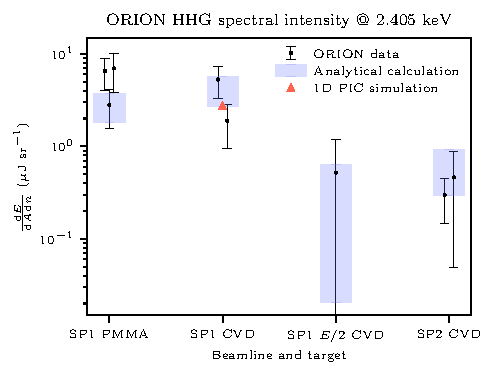
\includegraphics{figures/orion/orion_experiment_results}
	\caption[X-ray harmonic intensities measured on the ORION experiment compared to theory and simulation.]{\textbf{X-ray harmonic spectral intensities at 2.405 keV measured on the ORION experiment compared to theory and simulation.} The analytical calculation corresponds to the thick lines marked in Figure \ref{fig:orionintensitycurves}. The 1D PIC simulation result is derived from Figure \ref{fig:orionxrayharmonics} and scaled to the ORION laser pulse duration.}
	\label{fig:orionexperimentresults}
\end{figure}
Experimental data points are consistent within their errors with one another, the theory and the simulation, albeit with large uncertainties with such a low shot number. Notably, for the CVD targets, the SP1 beamline is on average almost 10 times brighter than the SP2 beamline despite the greater energy content and greater component of the laser pulse electric field directed into the plasma for the SP2 beamline. At the same time, the single beamlet shot is over 5 times weaker in intensity compared to the mean intensity of the full SP2 beamline. These highly non-linear scalings are consistent with HHG theory but cannot be understood to be from bremsstrahlung emission. 

Bremsstrahlung emission from steep density profile low-Z solid density targets irradiated by relativistic laser pulses remains an area of active research with experiments to explore this in the planning stages at the University of York. However, it is possible to derive approximate best-case scenario scalings of spectral intensity with incident energy. A plasma in equilibrium has a kinetic energy $E = 3/2 k_\mathrm{B}T$ \cite{chenIntroductionPlasmaPhysics2016}. In the ROM regime, energy absorption does not depend on incident energy, thus the plasma temperature increases linearly with incident energy. Now, assuming the target can be treated as a radiating black body, the spectral radiated intensity increases most rapidly with temperature when $h\nu \ll k_\mathrm{B}T$ at which point the spectral radiance scales linearly with temperature \cite{zangwillGuidedConfinedWaves2012}. Thus, in the best case, one could expect a linear increase in the spectral intensity measured from the double beamlet compared to the single if that signal originated from bremsstrahlung emission. Note further that this scaling depends not on the incident intensity but only on the incident energy, a well-constrained quantity on ORION.

The above discussion relied on the assumptions of equilibrium and a black-body radiation spectrum. While this is valid for the long radiating period after the main pulse interaction, in much of this thesis, emphasis has been placed on the non-equilibrium state of the interaction itself. There are two species of relevance during this time: the hot electrons around the front surface directly heated by the laser pulse and prepulse, and the hot electrons that are reflected specularly and are responsible for SHHG. In \cite{zulickHighResolutionBremsstrahlung2013}, bremsstrahlung of these species is measured experimentally for a 30 fs laser pulse and $a_0$ = 2.8. As the populations of each of these species are so small, the peak contribution to the photon spectrum is many orders of magnitude smaller than that of the experimental signal and can therefore be neglected.

Applying hole boring theory, the measured intensity of the SP2 beamline implies an energy $0.102_{ - 0.044}^{ + 0.1733}$\unit{\mu J} per harmonic at 2.405 keV, corresponding to a total efficiency of $2.04_{ - 0.86}^{ + 3.47}\times 10^{-10}$ into each harmonic at these photon energies. Due to harmonic source size shrinkage and the roll-off, the efficiency of the SP1 beamline will be significantly lower. Integrating over the full spectrum given the SP2 X-ray efficiency \cite{gordienkoCoherentFocusingHigh2005}, at the new focal position, the peak intensity is increased by a factor $1040^{+ 740}_{ - 290}$, corresponding to peak powers higher than any other light source globally at this time. This dramatic magnification at focus is not unrealistic and is indeed consistent with the literature. Vincenti \textit{et al} demonstrated a 3 order of magnitude gain for a 3 PW 20 fs system \cite{vincentiAchievingExtremeLight2019}. The lower power here is compensated by the longer duration. It is interesting that from Equation \ref{eq:orion-magnification}, for the ROM regime, the integration over the spectrum at the new focal spot contains a harmonic series that is only terminated by the roll-off. Thus, while simulations have demonstrated a gain of 1000 for a 3D simulation, it is unlikely that it had the necessary resolution to resolve the full peak in intensity and it could be notably higher.


Flying focus discussion here.

% Note that if you replace the spatial Gaussian with a sinc^2 profile with the same FWHM, they look almost identical to exponential. The spatial integral is approx 1.06 times larger thus minimal impact on the profile

\section{ \label{ch:3-sec:conclusion}Summary and discussion}
This chapter has described in full the experimental methods and results of the recent ORION SHHG experiment. The X-ray harmonic intensities were measured using the OHREX spectrometer. To describe the results, the ROM model of SHHG was applied, combining all pieces of the puzzle to reconstruct the measured intensities analytically. The experimental campaign was supported by PIC and hydrodynamic simulations of the main pulse and prepulse interactions respectively. PIC simulations agree with the analytical results for the ORION parameter space. No preplasma expansion was expected for the SP1 beamline and reasonable preplasma scale lengths for the SP2 beamline provided the addition of a single PM optic. Some discussion of plasma temperature was given.

The SP2 result is plotted in context with other laser systems in Figure \ref{fig:lasersystems}.
\begin{figure}
	\centering
	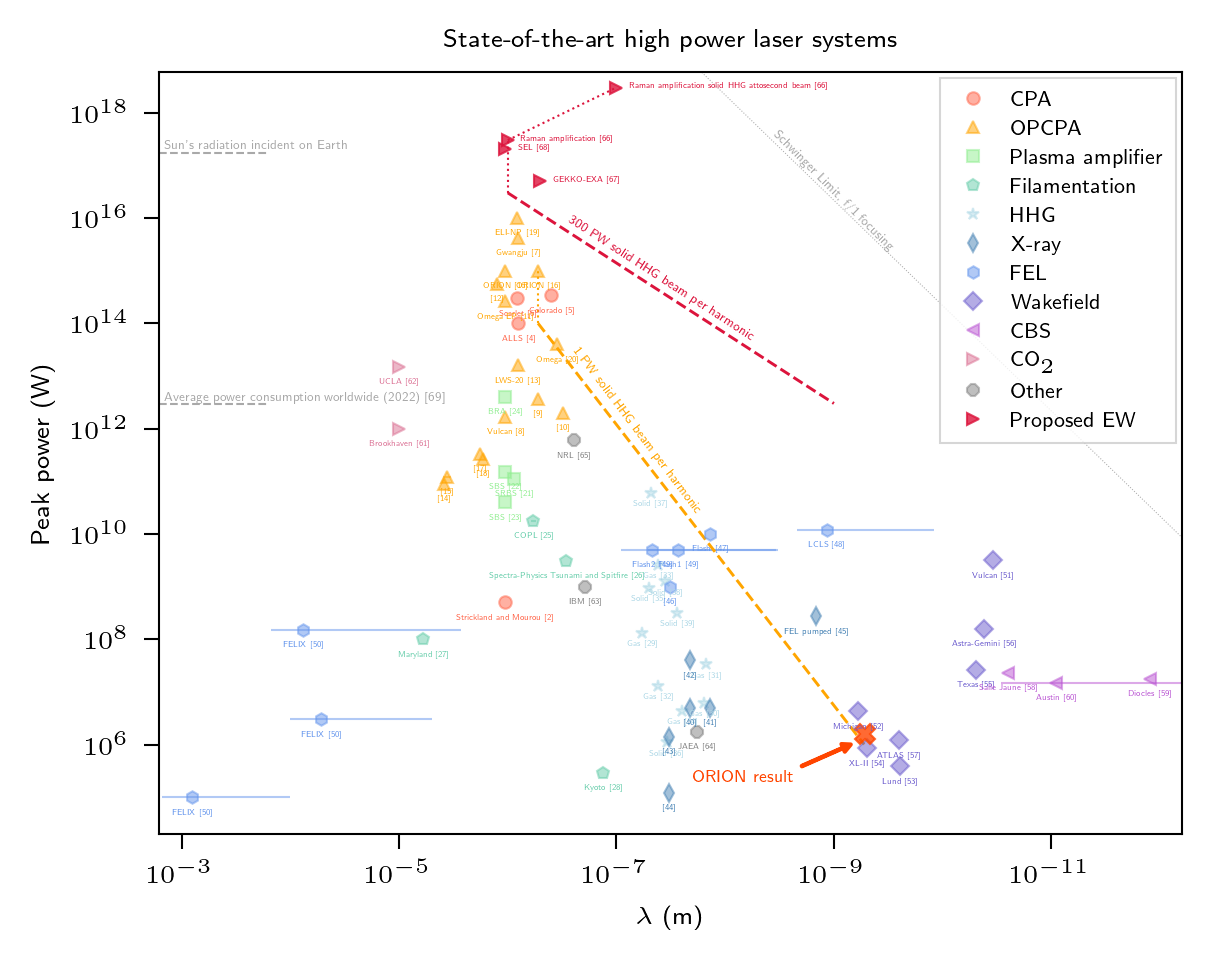
\includegraphics{figures/intro/laser_systems}
	\caption[The ORION result in context.]{The ORION SP2 result in context with other high power laser systems. This is the only measurement to date of the absolute intensity of XHHG. Dashed lines indicate the power of the ORION SHHG beam and the SHHG beam that could be anticipated from the use of a sub-exawatt scale facility as will soon become available.}
	\label{fig:lasersystems}
\end{figure}
The XHHG beam sits in the viscinity of betatron radiation from laser wakefield experiments. Betatron radiation, however, is typically on the order of a few femtoseconds in duration. The stated power of the XHHG beam is averaged over the entire laser pulse to enable comparison to the dashed line of ROM scaling. In reality, the duration of the X-ray radiation burst, from Figure \ref{fig:orionattosecondpulse}, is at most 30 as and the beam is broadband, corresponding to a peak power of at least \qty{2e10}{W.keV^{-1}}. This is comparable to the LCLS, the most power XFEL.
% approx 140 cycles in SP2 laser pulse
Figure \ref{fig:lasersystems} also highlights the power spectrum that could be obtained from a next-generation sub-etawatt facility as are being commisioned currently or could be produced via Raman Amplification \cite{trinesSimulationsEfficientRaman2011}. Simulations have suggested the Coherent Synchrotron Emission regime can be accessed for these laser pulse intensities up to the X-ray regime \cite{edwardsXRayEmissionEffectiveness2020}, hence the shallower scaling. Thus an entirely new parameter space becomes available both from the individual harmonics and for the conservative estimate of the intensity at the new focus. The figure is somewhat misleading with regard to the Schwinger Limit. This is for f/1 focusing. The RPM from an exawatt laser would have a must tighter focus and would access the Schwinger limit at the new focus. These exciting opportunities have contributed to the success of the recent proposal to study SHHG at GEMINI PW.

% TODO I must redo the boosted section since I made a mistake there and rethink a bit about optimum theta.
% TODO I must also at some point just state that a hat indicates a normalised vector.
% TODO READ https://www.nature.com/articles/s42005-024-01575-z
% TODO https://www.nature.com/articles/ncomms12515